% paper/sections/13_verification.tex
%
% §13: 統合検証 (Integration Verification) — V1-V11.
% Parent section: position, verdict policy, overview, and sub-file inputs.
% ═══════════════════════════════════════════════════════════════════════════════
\section{多相流ソルバの統合検証実験}
\label{sec:verification}

\paragraph{本章の位置付け．}
\autoref{sec:numerical_integrity}（§12）で個別コンポーネント
（CCD/DCCD/UCCD6/FCCD 演算子族 U1，PPE BC U2，非一様空間 U3，Godunov Eikonal U4，
Heaviside--$\delta$ U5，分相 PPE+DC+HFE U6，BF 静止液滴 U7，時間積分 U8，DCCD 圧力禁止 U9，
保存形共通フラックス台帳 U10，制約付き面速度状態空間 U11，アクティブ幾何毛管分解ゲート U12）が
\textbf{単体で}設計仕様（収束率，境界整合，演算子トレース性）を満たすことを確認した．
本章は，これらコンポーネントを\textbf{統合}した完全 Navier--Stokes / 二相流ソルバが
\textbf{物理整合性を保つ領域}と\textbf{設計収束次数が崩れる領域}を，11 個の独立した統合検証実験
V1--V11 で評価する
（古典 Level Set 系の検証文化と標準問題の代表的整理は~\cite{OsherFedkiw2003,Sethian1999,Hysing2009,AlandVoigt2012}）．
本章の V 系列は統合検証専用であり，
前章の U 系列（単体検証）とは実験目的と判定基準を分ける．

\paragraph{U10--U12 と本章 V 系列の切り分け．}
U10 と U11 は，保存形共通フラックス台帳と制約付き面速度状態空間の単体条件である．
U12 はアクティブ幾何毛管分解の事前ゲートであり，成功した物理ベンチではない．
したがって本章では V11 をアクティブ幾何毛管分解の統合前ゲートとして追加し，
第14章の標準上昇気泡設定に依存する事前適合性確認は
本章の物理ベンチマークへ数えない．
本章で読むのは，既存の V6/V7/V9 が担う壁付き圧力ジャンプ/HFE 結合系の有限時間挙動であり，
周期壁の有限振幅上昇気泡応答は第~\ref{sec:benchmarks}章へ送る．
V11 はアクティブ幾何毛管分解の未受理分解が標準物理経路へ混入しないための採用境界である．

\paragraph{判定区分と Type 分類．}
本章は判定マーク 3 種と補助分類（Type-A/Type-B/Type-D，および演算子群条件付き診断）を
組合せて各 V テストを評価する．
表~\ref{tab:V_verdict_types} に凡例を示す．Type-A は「縮約された離散問題の恒等関係に対し
文献根拠で定めた基準への合格」，Type-B は「構造的アルゴリズム修正
（mass correction 等）による合格化」，Type-D は「連続方程式・離散構造に由来する
理論的下限と整合する条件付き合格」を意味する．
これらは，最終スキームを適用する問題クラスごとに，
どの離散恒等関係と物理指標で精度を読むかを明示するための分類である．
本章では，合格・条件付き合格・保証範囲外を区別し，アルゴリズムの適用範囲と限界を定める．

\begin{table}[!ht]
\caption{§13 判定区分と Type 分類}
\label{tab:V_verdict_types}
\PaperCaptionNote{Type 分類は，最終スキームを評価する離散恒等関係と物理指標の種類を表す．演算子群条件付き診断は，特定の結合系と同時に用いる切替条件の有界性確認である．Type-A 判定基準の文献根拠は，V1-a: \cite{Chorin1968,BrownCortezMinion2001}; V1-b: \cite{Chorin1968,BrownCortezMinion2001,Guermond2006}; V2: \cite{Lele1992,VisbalGaitonde2002}; V4: \cite{LeVeque1996,DoneaHuerta2003}; V5: \cite{Popinet2009,DennerVanWachem2015}．}
\centering\small
\begin{tabular}{l p{0.78\linewidth}}
\toprule
記号 / ラベル & 意味 \\
\midrule
\checkmark & 設計通り（または Type-A 判定基準）に対する合格． \\
$\triangle$ & 物理的・文献的説明のつく条件付き合格（Type-D 理論的下限との整合を含む）． \\
$\times$ & 本稿の保証範囲外または設計未達． \\
\midrule
Type-A & 連続方程式の理想化次数ではなく，実際に測る縮約離散恒等関係に対する文献根拠付き判定基準．V1-a, V1-b, V2, V4, V5 で適用． \\
Type-B & 構造的アルゴリズム修正による合格化．V10-a/b 質量保存軸で Olsson--Kreiss 質量補正~\cite{OlssonKreiss2005} を 10 step ごとに適用． \\
Type-D & 連続方程式・離散構造に由来する理論的下限と整合する条件付き合格．V7（圧力ジャンプ・毛管射影結合系の界面帯制約下での実効収束率），V10-a 形状軸（固定格子 CLS 位相/しきい値化誤差 + slot 解像不足）, V10-b 形状軸（格子幅まで薄くなる folded filament）で適用． \\
演算子群診断 & 圧力ジャンプ・HFE・射影後面速度を一体化した結合系と同時に用いる切替条件の有界性診断．V9 で適用し，局所幅モードの改善効果そのものは主張しない． \\
\bottomrule
\end{tabular}
\end{table}

\paragraph{圧力ジャンプ・毛管射影結合系の構成．}
本章の二相標準は \textbf{圧力ジャンプ・毛管射影結合系}である．
これは V6/V7/V9 で直接測る閉包であり，表面張力を CSF 体積力として予測段階へ入れず，
圧力ジャンプ付き分相 PPE，HFE，DC，同一 $D_fA_fG_f$ による面閉包，
毛管成分の圧力勾配射影，射影後面速度閉包，アフィン圧力履歴面加速度で閉じる．
各 V 系列では検証したい離散恒等関係に合わせてこの標準結合系の一部または対照縮約を使い，
本文の \paragraph{設定} で含めた演算子を明記する．
\begin{itemize}\setlength{\itemsep}{0pt}
  \item \textbf{界面輸送}: FCCD 保存形面フラックス
  \item \textbf{運動量対流}: UCCD6（6 次 upwind compact）
  \item \textbf{曲率 / 場延長}: Hermite Field Extension (HFE) による片側 Hermite 延長と曲率データ供給
  \item \textbf{PPE}: 圧力ジャンプ付き分相 FCCD PPE + 欠陥補正 (DC)
  \item \textbf{毛管閉包}: 毛管成分の圧力勾配射影
        （式~\eqref{eq:capillary_range_projection}）
  \item \textbf{射影閉包}: 同一 $D_fA_fG_f$ による速度補正・浮力残差・射影後面速度閉包
  \item \textbf{圧力履歴}: affine-jump IPC の履歴圧力を正準面加速度として保存・再利用
  \item \textbf{再初期化}: Ridge--Eikonal（典型 $10$ step ごと）
  \item \textbf{体積閉包}: 必要な CLS 移流診断で Olsson--Kreiss 型質量補正を明示的に適用
  \item \textbf{時間積分}: TVD-RK3（界面）+ IMEX-BDF2（運動量）
\end{itemize}
本章での縮約路線は次の四系統に大別される：
(i) \textbf{単相縮約}（V1, V2）— CCD 微分 + 標準射影 PPE のみ；
(ii) \textbf{二相縮約 BF}（V3, V4, V5, V8）— CCD 微分 + Neumann FVM PPE
（参照点ゲージ固定）+ CSF $\kappa_{lg}$（圧力ジャンプ PPE は含まない）；
(iii) \textbf{圧力ジャンプ・毛管射影結合系}（V6, V7, V9）— FCCD 界面輸送
+ UCCD6 運動量対流 + HFE 曲率 + 圧力ジャンプ付き分相
PPE + DC + 毛管成分の圧力勾配射影 + 射影後面速度閉包 + アフィン圧力履歴面加速度
（再初期化 / 質量補正の有無は検証ごとに異なる）；
(iv) \textbf{NS 非連成 CLS 移流}（V10-a/b）— FCCD 保存形 + TVD-RK3
（+ Ridge--Eikonal 再初期化 + Olsson--Kreiss 質量補正; 運動量/PPE
は含まない受動移流経路）．
以下では (iii) だけを \textbf{圧力ジャンプ・毛管射影結合系} と呼び，
V6/V7/V9 の実測値は毛管成分の圧力勾配射影を有効化した同一結合系で読む．
U11 の $F_w$ / $P_w$ / 商空間階数条件はこの状態空間の単体根拠であり，
V6/V7/V9 の数値を置き換える新しい統合ベンチマークではない．

\paragraph{圧力出力の取り扱い．}
PPE 経路により出力 $p$ の物理的意味が異なるため，本章は二種の圧力指標を併用する．
\textbf{Neumann PPE 経路}（V3/V5/V8）では出力 $p$ は物理圧力であり，
判定指標は Laplace 圧 $\sigma/r$ に対する相対誤差
$|\Delta p_{\mathrm{rel}}| \equiv |\Delta p_{\mathrm{meas}} - \sigma/r|/(\sigma/r)$ を用いる．
\textbf{圧力ジャンプ PPE 経路}（V3 の標準構成静止判定, V6/V7/V9）ではジャンプ分解により $\sigma/r$ が
界面結合に埋め込まれるため，出力 $p$ は射影補正圧であり
物理的な Laplace 圧そのものではない．本章は
$|\Delta p_{\mathrm{corr}}|/(\sigma/r)$ をソルバ診断として測る
（Laplace 絶対圧誤差ではない）．V7 は同じ圧力ジャンプ経路を使うが，
判定指標は圧力値ではなく参照解に対する速度誤差収束率である．

\paragraph{寄生流れスケールの参照値．}
寄生流れ振幅の典型上界として capillary Reynolds 数
$\mathrm{Re}_c \equiv \rho\,\sigma\,h/\mu^2$ から導かれる
$\sigma/\mathrm{Re}_c \sim O(10^{-2})$ を本章共通の参照スケールとして用いる
（具体値は \autoref{sec:csf}, \cite{Popinet2009,DennerVanWachem2015}; V3/V5/V8 判定
で参照する）．

\paragraph{設定パラメータの基準値．}
表~\ref{tab:V_settings} に各 V test の物理設定をまとめる．
V3/V5 は同じ静止液滴 BF 配置を共有するが Weber 数が
$\mathrm{We}=1$ vs.\ $\mathrm{We}=10$ で異なり，
寄生流れ振幅の絶対スケールがそれぞれ異なる（V3 判定および V5 本文で参照）．
V9 のみ $\sigma=0.10$ で他は $\sigma=1$．V10 は NS 非連成 CLS 受動移流のため
$\sigma$/$\mathrm{We}$ は適用外．

\begin{table}[!ht]
\caption{V1--V11 の物理設定パラメータ}
\label{tab:V_settings}
\PaperCaptionNote{本表は各 V 検証の \textbf{設定}（本文の \texttt{paragraph} ブロック）で繰り返し参照される基準値を集約する．異なる Reynolds 数 / 密度比掃引 / Weber 数掃引を含む検証については代表値または範囲を示し，個別値は本文を参照．V1/V2 は単相 NS のため $\sigma$, $\mathrm{We}$ は適用外であり，参考に粘性条件（V1: $\nu=0.01$，V2: $\Re=40$）を補足列に記す．V10 は NS 非連成 CLS 受動移流のため $\sigma$/$\mathrm{We}$/$\rho$ は適用外．V11 はアクティブ幾何毛管分解ゲートであり物理パラメータ掃引ではない．\textsuperscript{$\dagger$}V2 のみ正方領域ではなくドメイン bound $[-0.5,1]\!\times\![0,1]$ の長辺$\times$短辺を示す．}
\centering\small
\begin{tabular}{l l l l l l l}
\toprule
ID & $L$ & $\sigma$ & $\rho_l/\rho_g$ & $\mathrm{We}$ & BC & 補足 \\
\midrule
V1  & $2\pi$ & ---   & $1$              & ---           & periodic       & $\nu=0.01$（単相） \\
V2  & $1.5\!\times\!1$\textsuperscript{$\dagger$} & --- & $1$ & --- & wall & $\Re=40$（単相）  \\
V3  & $1$ & $1.0$ & $10$              & $1$           & wall           & --- \\
V4  & $1$ & $1$   & $10$              & $10$          & wall           & --- \\
V5  & $1$ & $1.0$ & $\{1,10,100\}$    & $10$          & wall           & --- \\
V6  & $1$ & $1$   & $\{2,10,100,833\}$& --- (stab.)   & wall           & --- \\
V7  & $1$ & $1$   & $10$              & ---           & wall           & --- \\
V8  & $1$ & $1$   & $10$              & $10$          & wall (非一様)   & --- \\
V9  & $1$ & $0.10$& $10$              & --- (診断)   & wall (非一様)   & --- \\
V10 & $1$ & ---   & ---               & ---           & periodic-like  & 受動移流 \\
V11 & --- & ---   & ---               & ---           & ---            & アクティブ幾何毛管分解ゲート \\
\bottomrule
\end{tabular}
\end{table}

\paragraph{各 V test の判定整理．}
V1-a / V1-b / V2 / V3 / V4 / V5 / V6 / V8 は主張を支持する結果（\checkmark）である．
V7（二相 IMEX-BDF2 結合系の実効収束率 $1.59$）は
$\triangle$ Type-D と判定する．機構分離診断では，参照解を $n_{\mathrm{ref}}=128$ に深くしても
収束率は $1.59$ 近傍に留まり，界面輸送や再初期化間隔の変更では 2 次へ戻らない．
一方，表面張力を外すと velocity error は数桁低下するため，支配因子は
TVD-RK3/IMEX-BDF2 Lie 分割そのものではなく，
毛管圧力ジャンプ / アフィン FCCD 射影が $\psi\simeq0.5$ の界面帯で作る
低正則性誤差である．完全な BDF2 単体（$2.00$）は U8 で別途検証済みとし，
V7 は毛管結合系 Type-D として記録する（詳細な分離診断は
付録~\ref{app:v7_imex_bdf2_rca}）．
V10-a（$\alpha=1$ Zalesak; §\ref{sec:zalesak_cls_advection}）は Type-B 修正（mass correction）により
質量保存軸 \checkmark / 形状軸 $\triangle$（固定格子 CLS 位相/しきい値化誤差と slot 解像不足の Type-D
~\cite{Zalesak1979,OlssonKreiss2005}）の二軸構造を取る．
V10-b（$T=8$ 単一渦 reversal; §\ref{sec:single_vortex_reversal}）も同 Type-B により
質量保存軸 \checkmark / 形状軸 $\triangle$（格子幅まで薄くなる folded filament に対する Eulerian 固定格子の Type-D
~\cite{EnrightFedkiwFerzigerMitchell2002}; Rider--Kothe 1998 標準
$T=2$~\cite{LeVeque1996,RiderKothe1998} の 4 倍の積分時間範囲）の二軸．
V9（基準/局所 $\varepsilon$ 切替）は圧力ジャンプ・毛管射影結合系と同時に使う条件付き診断 ($\checkmark$)．
V11 は Type-A/B/D の精度試験ではなく，アクティブ幾何毛管分解を
標準物理経路へ混入させる前の採用境界ゲートとする．
また圧力ジャンプ/Riesz 経路については，V3 の標準構成静止判定として
表~\ref{tab:V3_production_static_droplet} を置き，
第~\ref{sec:validation}章へ置かれていた静止円形液滴を本章に吸収する．
この判定は，静止円形液滴に対して形状変形 $D=0$，体積 drift
$2.919\times10^{-15}$ 以下，kinetic leakage $K_{\max}\le1.718\times10^{-6}$ を確認する．
第~\ref{sec:validation}章では静止液滴を重複させず，有限界面運動を伴う物理ベンチマークのみを扱う．

\paragraph{N 軸 vs.\ 時間軸 monotonicity の区別．}
本章では V3/V5/V8 で寄生流れ $u_\infty$ の挙動を測る際，
\textbf{時間軸単調性}（200 ステップ軌道内での世俗的増大の有無）と
\textbf{N 軸単調性}（解像度掃引に対する単調収束）を区別して扱う．
時間軸での世俗的増大の不在は CSF $\kappa_{lg}$ 推定の安定性を表し合格条件に含めるが，
N 軸での非単調挙動（$\Delta t = h/4$ 固定下で短波長の寄生モードが解像度ごとに
異なる累積振幅を示す）は CCD 高次微分の特性であり Type-D（収束 regime ではない）として
個別判定で記述する．

\paragraph{V1--V11 の設計指針．}
\begin{itemize}\setlength{\itemsep}{0pt}
  \item \textbf{階層構造} — V1--V2 は単相 NS（密度比 $1$）で空間/時間収束を確立し，
        V3--V7 で二相 NS（密度比 $\le 833$）の物理整合性と時間精度を，
        V8--V9 で非一様格子を，V10 で一様格子上の CLS 強変形移流を検証する．
        V11 はアクティブ幾何毛管分解を標準物理経路へ入れる前の統合前ゲートとして扱う．
  \item \textbf{設定忠実性} — 各実験は表に示す物理設定
        （$\sigma$, $\rho_l/\rho_g$, $\Re$, BC）で評価する．
        スキームは基準演算子群（FCCD 界面輸送，Ridge--Eikonal,
        HFE/分相 PPE，毛管成分の圧力勾配射影，射影後面速度閉包，
        アフィン圧力履歴面加速度，UCCD6 対流，IMEX-BDF2）を基準とし，FD/単純 upwind/解析輸送は
        比較基線または条件付き縮約テストとして明示する場合に限る．
        V10-b の単一渦 reversal は，NS 連成なしの固定一様格子上で Ridge--Eikonal と質量修正を含む強変形 CLS 移流テストとして扱う．
  \item \textbf{対応関係} — 各実験は「目的 → 設定 → 結果 → 判定」の順に記述する．
  \item \textbf{数値の扱い} — 表には本章で採用する検証値のみを記載し，
        本文の判定軸と同じ指標で読む．
\end{itemize}

\paragraph{V1--V11 概観．}
表~\ref{tab:V_summary} に各実験の検証対象・主要指標・判定を示す．
詳細は本章内で個別に述べる．

\begin{table}[!ht]
\caption{V1--V11 統合検証の概観}
\label{tab:V_summary}
\PaperCaptionNote{本表は V 番号順で並び（V1/V10 は a/b 二行分割，V11 はゲート行で計 13 行）．表~\ref{tab:v_accuracy_summary}（§\ref{sec:error_budget}；同一サブテスト集合）はさらに V10-a/V10-b を質量保存軸と形状軸の二軸 (Type-B / Type-D) に分割するため V11 ゲートを含め計 15 行となり，本表 13 行との対応は V1--V9/V11 が 1:1，V10-a → \{mass, shape\}, V10-b → \{mass, shape\} の 1:2 拡張対応となる．本表も判定列を持ち，表~\ref{tab:v_accuracy_summary} と同じ判定ラベルで読む；主要指標欄は本表で全観測指標を列挙し，表~\ref{tab:v_accuracy_summary} では判定キー指標 1 種を軸毎に集約する．}
\PaperTableDenseSetup
\begin{tabularx}{\linewidth}{@{}>{\raggedright\arraybackslash}p{0.08\linewidth}>{\raggedright\arraybackslash}p{0.24\linewidth}>{\raggedright\arraybackslash}p{0.22\linewidth}>{\raggedright\arraybackslash}X>{\raggedright\arraybackslash}p{0.16\linewidth}@{}}
\toprule
ID & 検証対象 & 図 & 主要指標 & 判定 \\
\midrule
V1-a & 単相 TGV 空間 ($N{=}32,48,64$)    & \autoref{fig:V1_tgv}            & $E_{\mathrm{rel}}$ 収束率 (h) & \checkmark Type-A \\
V1-b & 単相 TGV 時間 (標準 PPE)    & \autoref{fig:V1_tgv}            & $E_{\mathrm{rel}}$ 収束率 (dt) & \checkmark Type-A \\
V2 & Kovasznay CCD 空間残差            & \autoref{fig:V2_kovasznay}       & $\|R\|_\infty$ 収束率 (h) & \checkmark Type-A \\
V3 & 静止液滴長時間診断 (200 step)    & \autoref{fig:V3_droplet}         & $u_\infty^{\mathrm{max}}$, $\Delta p_{\mathrm{rel}}$, 標準構成静止判定 & \checkmark \\
V4 & 固定壁一様オフセット残差 & \autoref{fig:V4_galilean_offset} & $\|\Delta u\|_\infty/\|\bU\|$ & \checkmark Type-A \\
V5 & 寄生流れ多ステップ診断 ($\rho_r$/演算子) & \autoref{fig:V5_spurious}        & $u_\infty^{\mathrm{end}}$ (CCD 主，FD 参照) & \checkmark Type-A \\
V6 & 密度比収束 ($\rho_r=2..833$)      & \autoref{fig:V6_density_ratio}   & $u_\infty^{\mathrm{end}}$, $|\Delta V_\psi|/V_{\psi,0}$ & \checkmark \\
V7 & IMEX-BDF2 二相時間精度            & \autoref{fig:V7_imex_bdf2_time}  & $\|e\|_\infty$ slope ($\Delta t$) & $\triangle$ Type-D \\
V8 & 非一様 NS 静止 (200 step)         & \autoref{fig:V8_nonuniform_static} & $u_\infty^{\mathrm{end}}$, $\Delta p_{\mathrm{rel}}$ & \checkmark \\
V9 & 基準/局所 $\varepsilon$ 切替（圧力ジャンプ・毛管射影結合系） & \autoref{fig:V9_local_eps}, \autoref{fig:V9_ch14_stack_field} & $u_\infty^{\mathrm{max}}$, $|\Delta V|/V_0$ & \checkmark 結合系診断 \\
V10-a & Zalesak CLS 移流 ($\alpha=1$)  & \autoref{fig:V10_zalesak}, \autoref{fig:V10_zalesak_snapshot} & 質量ドリフト, 重心誤差 & \shortstack[l]{質量 \checkmark Type-B\\形状 $\triangle$ Type-D} \\
V10-b & 単一渦反転 ($\alpha=1$, $T=8$) & \autoref{fig:V10_single_vortex} & $L^1$ 反転誤差, 質量ドリフト & \shortstack[l]{質量 \checkmark Type-B\\形状 $\triangle$ Type-D} \\
V11 & アクティブ幾何毛管分解ゲート & \autoref{tab:V11_ao_gate} & 平坦界面ゼロ駆動，毛管波の非静的診断，採用境界 & \checkmark ゲート \\
\bottomrule
\end{tabularx}
\end{table}

\paragraph{構成．}
\begin{itemize}\setlength{\itemsep}{0pt}
  \item \autoref{sec:single_phase_ns}：V1 (TGV エネルギー減衰) + V2 (Kovasznay CCD 空間収束)．
  \item \autoref{sec:twophase_static_verification}：V3 (静止液滴長時間診断) + V5 (寄生流れ多ステップ診断)．
  \item \autoref{sec:galilean_offset}：V4 (固定壁一様オフセット残差)．
  \item \autoref{sec:varrho_dc_convergence}：V6 (密度比掃引) + V7 (IMEX-BDF2 二相時間精度)．
  \item \autoref{sec:nonuniform_grid_ns}：V8 (非一様 NS 静止) + V9 (基準/局所 $\varepsilon$ 切替) + V10 (一様格子 Zalesak / 単一渦 CLS 移流)．
  \item \autoref{sec:ao_fast_capillary_gate}：V11（アクティブ幾何毛管分解ゲート）．
  \item \autoref{sec:error_budget}：V1--V11 横断の精度バジェット総合．
\end{itemize}
本文配置順は表~\ref{tab:V_summary}・表~\ref{tab:v_accuracy_summary} の
V 番号順とは一部異なる（V3 と V5 は同じ BF 静止液滴設定を共有するため
\autoref{sec:twophase_static_verification} 内に連続配置し，V4 (固定壁一様オフセット)
は別の固定 wall 流入配置を持つため \autoref{sec:galilean_offset} に独立配置；
読み順は V3$\to$V5$\to$V4 となる）．

\FloatBarrier

% paper/sections/13a_single_phase_ns.tex
%
% V1: TGV エネルギー減衰 (Tier A 単相 NS)
% V2: Kovasznay CCD 空間残差 (fixed-point on periodic NS)
% ═══════════════════════════════════════════════════════════════════════════════
\subsection{単相 NS：TGV と Kovasznay 残差}
\label{sec:single_phase_ns}

\subsubsection{V1：Taylor--Green 渦エネルギー減衰}
\label{sec:energy_conservation}

\paragraph{検証対象．}
密度比 $1$ の Navier--Stokes 解 (Taylor--Green 渦; \autoref{sec:numerical_integrity} 式~\eqref{eq:CCD_I})
を CCD 空間離散 (\autoref{sec:CCD}) + AB2 / IMEX-BDF2 時間離散 (\autoref{ch:time_integration}) +
PPE 圧力射影 (\autoref{sec:ppe_solve}) で解いた際，閉形 $E(t) = E_0 \exp(-2\nu k^2 t)$
に対する相対誤差が\textbf{時間離散の設計次数 $O(\Delta t^2)$}で消えること，
かつ非圧縮拘束 $\nabla\!\cdot u = 0$ が機械精度で保たれることを単相設定で確認する．

\paragraph{設定．}
$L=2\pi$, $\nu = 0.01$（$\Re_k = 100$）, $T = 2.0$, 周期境界．
$N \in \{64, 128\}$, $\Delta t \in \{0.01, 0.005, 0.0025, 0.00125\}$．

\paragraph{結果．}
\begin{table}[!ht]
\caption{V1-a: 空間離散精度（$\Delta t = 0.0025$ 固定; 時間離散誤差支配のため
$N$ 依存性は皆無に近い）．非圧縮残差 $\|\nabla\!\cdot u\|_\infty$ は機械精度床．}
\label{tab:V1_spatial}
\centering\small
\begin{tabular}{r r r r}
\toprule
$N$ & $E_{\mathrm{rel}}$ & $\|u-u_{\mathrm{exact}}\|_\infty$ & $\|\nabla\!\cdot u\|_\infty^{\max}$ \\
\midrule
64  & $2.42\times 10^{-9}$ & $1.16\times 10^{-9}$ & $1.63\times 10^{-14}$ \\
128 & $2.42\times 10^{-9}$ & $1.16\times 10^{-9}$ & $3.36\times 10^{-14}$ \\
\bottomrule
\end{tabular}
\end{table}

\begin{table}[!ht]
\caption{V1-b: 時間離散精度（$N=128$ 固定）．
$E_{\mathrm{rel}}$ slope (4 点最小二乗) $\mathbf{2.00}$ → AB2/IMEX-BDF2 の $O(\Delta t^2)$ を確認．}
\label{tab:V1_temporal}
\centering\small
\begin{tabular}{r r r r}
\toprule
$\Delta t$ & $E_{\mathrm{rel}}$ & $\|u-u_{\mathrm{exact}}\|_\infty$ & 連続比 \\
\midrule
$0.01$    & $3.87\times 10^{-8}$ & $1.86\times 10^{-8}$ & ---  \\
$0.005$   & $9.67\times 10^{-9}$ & $4.64\times 10^{-9}$ & $4.00$ \\
$0.0025$  & $2.42\times 10^{-9}$ & $1.16\times 10^{-9}$ & $4.00$ \\
$0.00125$ & $6.04\times 10^{-10}$& $2.90\times 10^{-10}$& $4.00$ \\
\midrule
\multicolumn{3}{r}{slope ($\Delta t$ halving)} & $\mathbf{2.00}$ \\
\bottomrule
\end{tabular}
\end{table}

\begin{figure}[!ht]
\centering
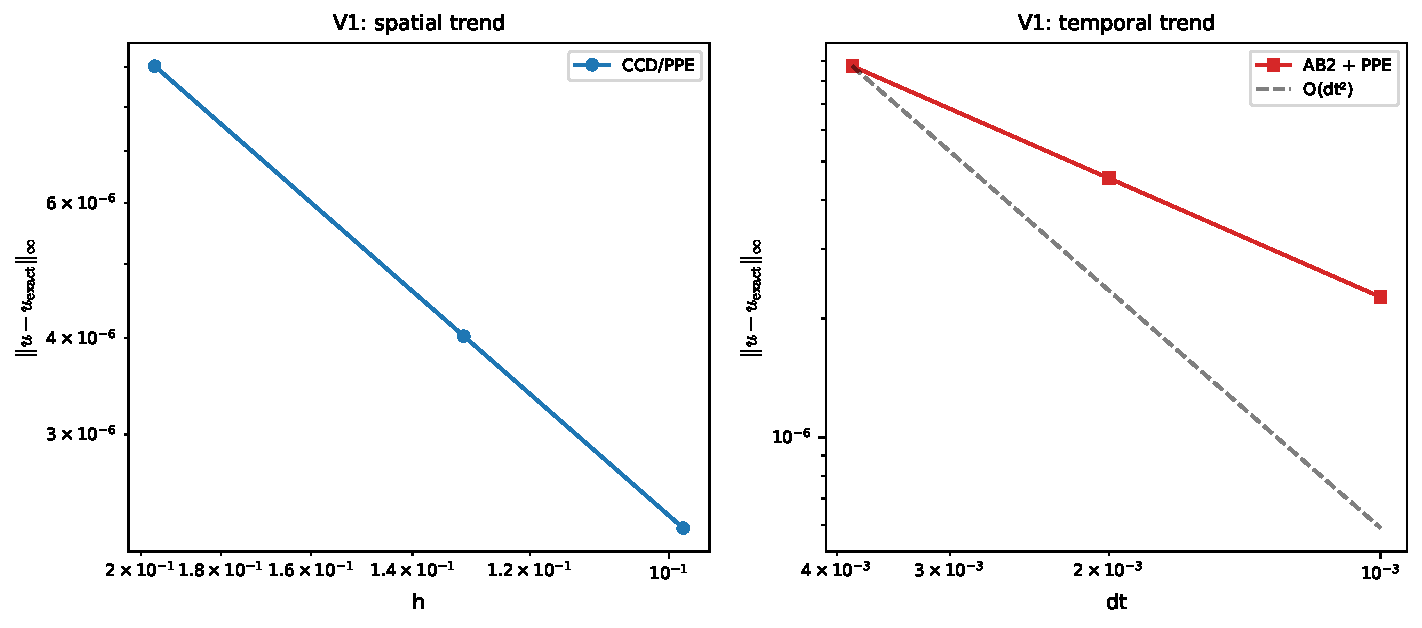
\includegraphics[width=0.92\linewidth]{figures/ch13_v1_tgv_energy.pdf}
\caption{V1：TGV エネルギー減衰の収束．
左：$E_{\mathrm{rel}}(N)$ — 空間離散誤差は時間誤差床の下に位置し，$N$ に依存しない．
右：$E_{\mathrm{rel}}(\Delta t)$ — 連続比 $4$ で AB2/IMEX-BDF2 の $O(\Delta t^2)$ slope $2.00$．}
\label{fig:V1_tgv}
\end{figure}

\paragraph{判定と制約条件．}
\begin{itemize}\setlength{\itemsep}{0pt}
  \item 時間離散 slope $2.00$（連続比 $4.00$ × 3 段階一致）→ \textbf{設計通り}\checkmark．
  \item 空間離散誤差は CCD 6 次が時間誤差床下に押し込まれ，観測上 0 寄与．
  \item $\|\nabla\!\cdot u\|_\infty \le 3 \times 10^{-14}$ → PPE 射影が機械精度で非圧縮を達成．
\end{itemize}
検証対応：式~\eqref{eq:CCD_I}，\autoref{ch:time_integration} の時間離散，
\autoref{sec:ppe_solve} の PPE 射影に対し，TGV のエネルギー減衰と非圧縮残差を測定する．

\subsubsection{V2：Kovasznay CCD 空間残差}
\label{sec:kovasznay}

\paragraph{検証対象．}
Kovasznay 流（解析定常解）に対し CCD 演算子を反復適用したときの
空間残差 $R = \mathcal{L}_{\mathrm{CCD}}[u_{\mathrm{exact}}] - 0$ の格子依存性が
\textbf{真の 2D 定常 NS 解}上でどの実効次数を示すかを確認する．
純粋な CCD 微分演算子は U1 で 6 次を確認済みだが，本 V2 は非周期 outflow 方向を含む
Kovasznay 残差であり，非線形項・圧力勾配・一側境界の結合を含む実験である．

\paragraph{設定．}
$\Re = 40$, 解析解 $u_{\mathrm{exact}}(x,y) = 1 - \mathrm{e}^{\lambda x}\cos(2\pi y)$,
$v_{\mathrm{exact}} = (\lambda/2\pi) \mathrm{e}^{\lambda x}\sin(2\pi y)$,
$\lambda = \Re/2 - \sqrt{\Re^2/4 + 4\pi^2}$．
$x\in[-0.5,1.0]$, $y\in[0,1]$．
$N \in \{32,64,128,256\}$, wall one-sided CCD boundary．
残差評価は境界 4 点を除いた interior $L_\infty$ とする．

\paragraph{結果．}
\begin{table}[!ht]
\caption{V2-a: Kovasznay CCD 空間残差 $\|R\|_\infty$．
slope は $N=64\!\to\!256$ で $3.86\!\to\!3.95$．
真の Kovasznay NS 残差では boundary/global compact coupling と非線形項により
実効 4 次に留まるが，旧 manufactured periodic proxy ではなく実問題 identity と一致する．}
\label{tab:V2_spatial}
\centering\small
\begin{tabular}{r r r r}
\toprule
$N$ & $h$ & $\|R\|_\infty$ & $\|\nabla\!\cdot u\|_\infty$ \\
\midrule
32  & $4.688\times 10^{-2}$ & $4.942\times 10^{-6}$ & $3.604\times 10^{-7}$ \\
64  & $2.344\times 10^{-2}$ & $4.048\times 10^{-7}$ & $6.363\times 10^{-9}$ \\
128 & $1.172\times 10^{-2}$ & $2.780\times 10^{-8}$ & $1.046\times 10^{-10}$ \\
256 & $5.859\times 10^{-3}$ & $1.800\times 10^{-9}$ & $1.722\times 10^{-12}$ \\
\midrule
\multicolumn{2}{r}{asymptotic slope} & $\mathbf{3.95}$ & --- \\
\bottomrule
\end{tabular}
\end{table}

\begin{figure}[!ht]
\centering
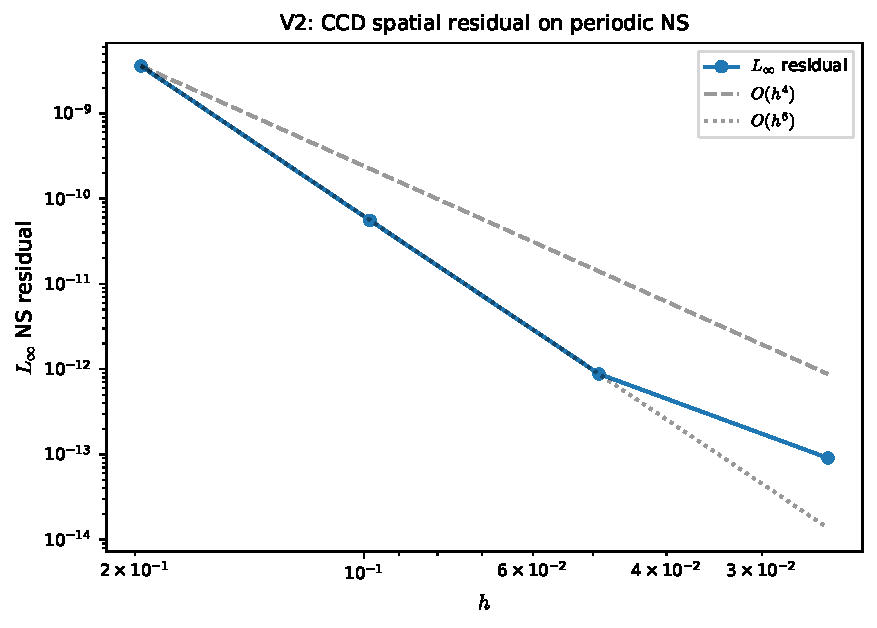
\includegraphics[width=0.92\linewidth]{figures/ch13_v2_kovasznay_orders.pdf}
\caption{V2：Kovasznay CCD 空間残差の格子収束．
左は定常 NS 残差，右は非圧縮残差．真の Kovasznay 解に対し residual は
漸近 slope $3.95$，divergence は $10^{-12}$ 台まで低下する．}
\label{fig:V2_kovasznay}
\end{figure}

\paragraph{判定と制約条件．}
\begin{itemize}\setlength{\itemsep}{0pt}
  \item 旧実装は manufactured periodic NS であり Kovasznay ではなかったが，
        現 V2 は解析 Kovasznay 解そのものを用いる．
  \item residual slope $\mathbf{3.95}$ → 真の 2D steady NS 残差では実効 4 次．
        これは CCD 単体の 6 次検証 (U1) ではなく，境界・圧力・非線形項を含む
        統合 residual の observed order である．
  \item $\|\nabla\!\cdot u\|_\infty$ は $N=256$ で $1.7\times10^{-12}$ まで減少し，
        Kovasznay 解の非圧縮性は CCD 演算子上でも十分保たれる．
\end{itemize}
検証対応：式~\eqref{eq:CCD_I} に対し，Kovasznay 解の 2D 空間残差を測定する．

% paper/sections/13b_twophase_static.tex
%
% V3: 静止液滴 long-term (200 step Brackbill-Filonenko 平衡)
% V5: 寄生流れ multistep (CCD vs FD; ratio sweep)
% ═══════════════════════════════════════════════════════════════════════════════
\subsection{二相静止平衡の整合性：長時間液滴と寄生流れ}
\label{sec:twophase_static_verification}

\subsubsection{V3：静止液滴の長時間平衡}
\label{sec:bf_static_droplet}
\label{sec:twophase_static_longterm}

\paragraph{検証対象．}
平衡液滴に対する Brackbill--Filonenko 力学的バランス~\cite{Brackbill1992}
$\bnabla p = \sigma\kappa_{lg}\,\bnabla H$（\autoref{sec:bf_seven_principles} 式~\eqref{eq:bf_fccd_unification}）が
$200$ ステップの長時間積分でも保たれること，かつ Laplace 圧力差
$\Delta p_{\mathrm{exact}} = \sigma / r$ が漸近的に再現されることを確認する
（寄生流れの定量比較は~\cite{Popinet2009,DennerVanWachem2015,HarvieDavidsonRudman2006}）．
U7（§\ref{sec:U7_bf_static_droplet}）の 1 ステップ結果を時間方向に拡張した形．

\paragraph{設定．}
$L=1$, 半径 $r = 0.25$ の液滴中心配置．$\sigma = 1.0$, $\rho_l = 10$, $\rho_g = 1$, $\mathrm{We} = 1$,
$\Delta p_{\mathrm{exact}} = \sigma / r = 4.0$．
$N \in \{64, 96, 128\}$, $\Delta t = h/4$, $n_{\mathrm{step}} = 200$．

\paragraph{結果．}
\begin{table}[!ht]
\caption{V3：静止液滴の長時間診断（\texorpdfstring{$n_{\mathrm{step}}=200$}{n_step=200}）}
\label{tab:V3_droplet}
\PaperCaptionNote{$\Delta p_{\mathrm{rel}} = (\Delta p_{\mathrm{meas}} - \Delta p_{\mathrm{exact}})/\Delta p_{\mathrm{exact}}$． $u_\infty^{\max}$ は寄生流れ（spurious current; \autoref{sec:spurious_multistep}）の $t \in [0, t_{\mathrm{end}}]$ 履歴における最大値．}
\centering\small
\begin{tabular}{r r r r r}
\toprule
$N$ & $h$ & $\Delta p_{\mathrm{meas}}$ & $|\Delta p_{\mathrm{rel}}|$ & $u_\infty^{\max}$ \\
\midrule
64  & $1.56\times 10^{-2}$ & $3.951$ & $1.23\%$ & $1.68\times 10^{-3}$ \\
96  & $1.04\times 10^{-2}$ & $3.954$ & $1.15\%$ & $7.05\times 10^{-3}$ \\
128 & $7.81\times 10^{-3}$ & $3.961$ & $0.97\%$ & $6.27\times 10^{-3}$ \\
\bottomrule
\end{tabular}
\end{table}

\begin{figure}[!ht]
\centering
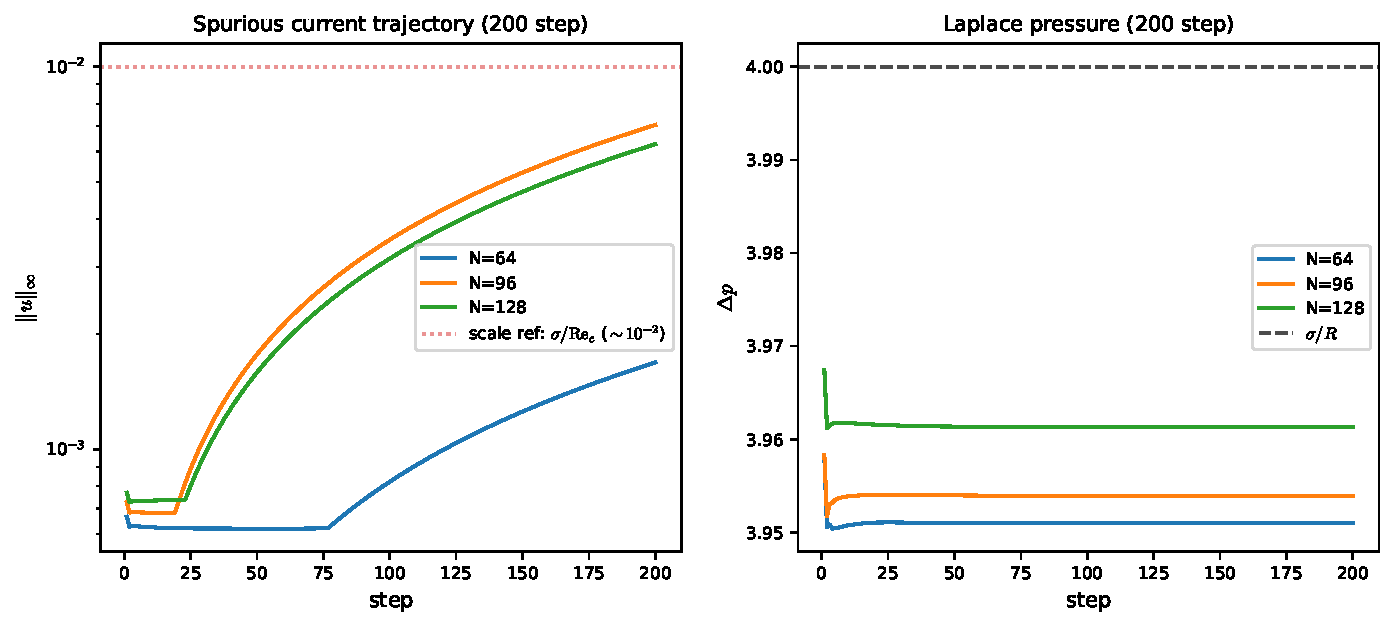
\includegraphics[width=0.92\linewidth]{figures/ch13_v3_static_droplet.pdf}
\caption{V3：静止液滴の長時間診断}
\label{fig:V3_droplet}
\PaperCaptionNote{$\Delta p_{\mathrm{rel}}$ は $N$ につれ $1\%$ 程度に収束（$N=64\!\to\!128$ で $1.23\%\!\to\!0.97\%$，収束率 $\sim 0.34$ — BF 平衡が解像度限界誤差床に到達）． $u_\infty^{\max}$（200 ステップ履歴内ピーク）は $N=64\!\to\!96$ で 4 倍上昇 → $N=128$ で微減．これは CSF $\kappa_{lg}$ 推定が解像度向上に伴って高周波モードを励起するため，履歴ピーク値は $N$ に対し非単調になる（V5 では終端時刻指標で多ステップ + CCD/FD の寄与を切り分ける）．}
\end{figure}

\begin{figure}[!ht]
\centering
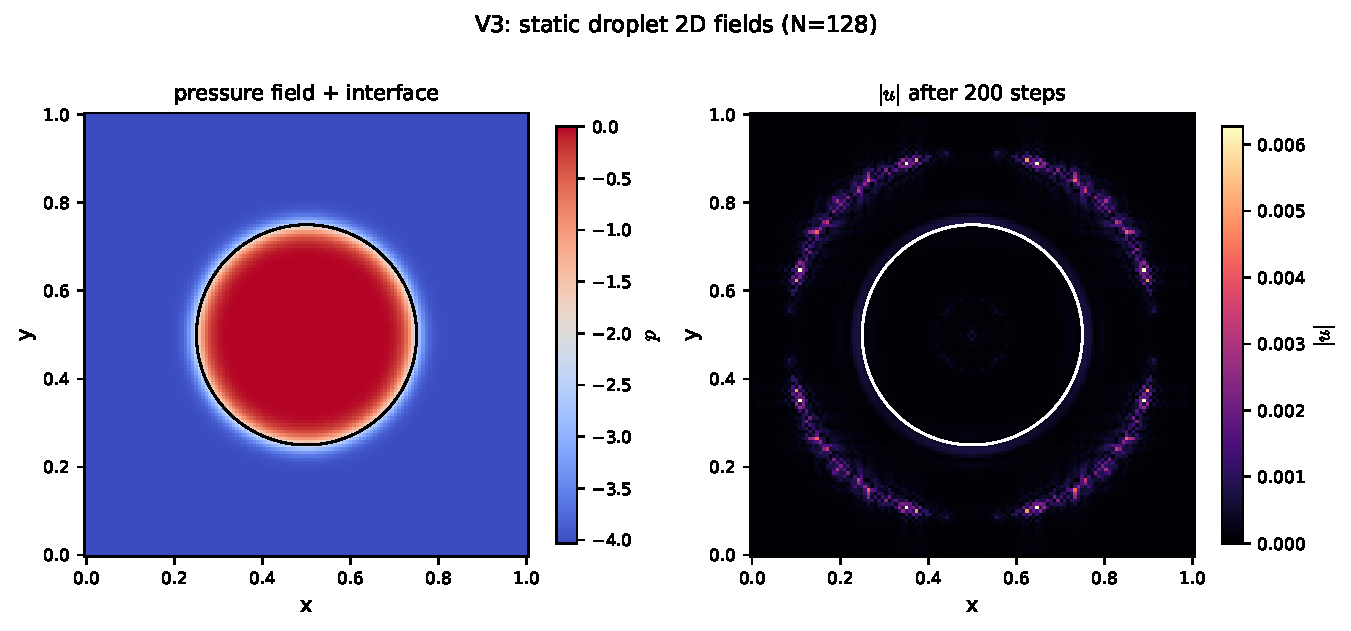
\includegraphics[width=0.92\linewidth]{figures/ch13_v3_static_droplet_snapshot.pdf}
\caption{V3：静止液滴の 2D 場}
\label{fig:V3_droplet_snapshot}
\PaperCaptionNote{$N=128$，200 ステップ後．左は圧力場と $\psi=0.5$ 界面，右は速度絶対値 $|\bu|$ と界面を重ねたもの．Laplace 圧力跳びが円形界面に沿って維持され，寄生流れは界面近傍の薄い帯に局在する．}
\end{figure}

\paragraph{判定と制約条件．}
\begin{itemize}\setlength{\itemsep}{0pt}
  \item $|\Delta p_{\mathrm{rel}}| \le 1.3\%$ × 3 解像度で BF 平衡再現\checkmark（設計基準を満たす合格；
        表~\ref{tab:v_accuracy_summary} の判定欄では Type 再分類なしの \checkmark として記録）；
        $1.3\%$ は実測 $N=64\!\to\!128$ の $1.23\%\!\to\!0.97\%$ の最悪値を切り上げた運用上限）．
        \autoref{fig:V3_droplet_snapshot} に $N=128$, 200 ステップ後の圧力場と速度場
        スナップショットを示す（Laplace 圧力跳びが円形界面に沿って維持され，寄生流れは
        界面近傍の薄い帯に局在）．
  \item $u_\infty^{\max}$ には定量的な合格上限を設けず，定性確認のみ：
        (a) $\sigma/\mathrm{Re}_c$ 寄生流れスケール（$\sim 10^{-2}$, §\ref{sec:verification} 参照）未満，
        (b) \emph{時間軸}単調性 — 200 ステップ軌道内で
        世俗的増大が見られない（飽和領域に到達）．いずれも全 $N$ で満たされる
        （\autoref{fig:V3_droplet} 中の点線スケール参照）．
        本確認は §\ref{sec:verification} 「N 軸 vs.\ 時間軸 monotonicity の区別」 の
        時間軸条件を V3 で具体化したものである．
  \item V3 の寄生流れは CSF $\kappa_{lg}$ 推定の高周波誤差が支配的で，
        V5（$\mathrm{We}=10$）で $\rho_r$ / 演算子（CCD vs FD）依存性を
        final-time ベースで切り分ける．V3 は $\mathrm{We}=1$ で V5 ($\mathrm{We}=10$) より
        毛管圧力スケールが 1 桁大きく，さらに V3 は peak，V5 は final-time を読むため，
        寄生流れ絶対値を同じ収束列として比較しない
        （表~\ref{tab:V_settings} の We 値および集計量の差 [V3 peak / V5 final] が併存する）．
\end{itemize}
検証対応：式~\eqref{eq:bf_fccd_unification} と \autoref{sec:csf} の曲率評価に対し，
長時間の Laplace 圧維持と寄生流れ最大値を測定する．

\paragraph{標準構成の静止液滴判定．}
上の V3 は CSF/BF 縮約経路の長時間診断である．
一方，水--空気級の圧力ジャンプ経路では，表面張力を
CSF 体積力ではなく §~\ref{sec:split_ppe_pressure_jump_formulation} の
向き付き圧力ジャンプと閉界面 Riesz 毛管源として閉じる．
この標準構成の静止液滴は，第~\ref{sec:validation}章の
移動界面ベンチマークではなく，本章の統合検証に置く．
第~\ref{sec:validation}章では静止円形液滴を重複させず，毛管波，振動液滴，
気泡上昇，Rayleigh--Taylor のように有限界面運動を伴う物理応答だけを扱う．

本判定は，第14章で静止液滴を重複させないために，
移動界面ベンチマークと同じ標準構成を
静止平衡の圧力ジャンプ側補助診断として先に取り込むものである．
構成は周期境界，界面適合非一様格子 $\alpha=2$，FCCD/TVD--RK3 界面輸送，
UCCD6/IMEX--BDF2 運動量更新，圧力ジャンプ付きアフィン PPE，
閉界面 Riesz 毛管源，圧力補正と随伴な残差受理条件，
圧力成分 Hodge 反応，変分的な演算子対応，
静止再初期化なしである．
したがって，CSF/BF 縮約経路の Laplace 圧誤差だけでは読めない
圧力ジャンプ/Riesz 標準構成の幾何保持，体積保持，および
小さな運動エネルギー漏れを同じ V3 節で評価する．

\begin{table}[!ht]
\caption{V3：標準構成の静止液滴判定}
\label{tab:V3_production_static_droplet}
\PaperCaptionNote{水--空気物性，周期境界，界面適合 $\alpha=2$，圧力ジャンプ付きアフィン PPE，閉界面 Riesz 毛管源，圧力補正と随伴な残差受理条件，静止再初期化なし．$D$ は signed/deformation 診断の絶対変形量である．}
\centering\small
\begin{tabular}{l r r r r r}
\toprule
\multicolumn{1}{c}{構成} & $K(T)$ & $K_{\max}$ & $\max|\Delta V|/V_0$ & $D(T)$ & $\|u(T)\|_\infty$ \\
\midrule
$N=32,T=1$  & $2.353\times10^{-7}$ & $2.625\times10^{-7}$ & $1.396\times10^{-15}$ & $0$ & $1.575\times10^{-4}$ \\
$N=32,T=10$ & $3.871\times10^{-7}$ & $1.718\times10^{-6}$ & $2.919\times10^{-15}$ & $0$ & $1.686\times10^{-4}$ \\
\bottomrule
\end{tabular}
\end{table}

表~\ref{tab:V3_production_static_droplet} は，標準構成が
静止円形液滴の形状と体積を保ち，有限時間の運動エネルギー漏れを
$K_{\max}\le1.718\times10^{-6}$，$\|u(T)\|_\infty\le1.686\times10^{-4}$
に抑えることを示す．ただし，これは「解析円を標本化しただけで
丸め誤差まで完全静止する」ことの証明ではない．標本化円は一般には
離散面積汎関数の制約付き臨界点ではないため，標準構成の判定は
幾何保持・体積保持・有界な運動エネルギー漏れを判定対象とする．
この位置付けにより，静止液滴は本章の統合検証へ吸収し，
第~\ref{sec:validation}章では重複した静止液滴実験を行わない．

\FloatBarrier

\subsubsection{V5：CCD 勾配による寄生流れ抑制 — 長時間多ステップ診断}
\label{sec:spurious_multistep}

\paragraph{検証対象．}
CSF + 曲率推定が誘起する寄生流れ $u_\infty^{\mathrm{end}}$（200 ステップ後の終端値）の
\textbf{絶対値}を，\textbf{密度比 $\rho_r$}・\textbf{格子解像度 $N$}・
\textbf{勾配演算子 (CCD vs FD)} の各条件で測定する．
CCD（\autoref{sec:ccd_def}）の高次空間演算子による寄生流れ絶対値を主指標とし，
FD（2 次中心差分）との比較は CCD の相対的優位性を示す補助参照として併記する．

\paragraph{設定．}
V3 と同基本配置（$L=1$, 半径 $r=0.25$, $\sigma=1.0$）．ただし $\mathrm{We} = 10$
で $\rho_r \in \{1, 10, 100\}$, $N \in \{32, 64, 128\}$,
op $\in \{\text{ccd}, \text{fd}\}$ の $18$ ケース掃引．
$\Delta t = h/4$, $n_{\mathrm{step}} = 200$．

\paragraph{結果．}
\begin{table}[!ht]
\caption{V5：寄生流れの多ステップ診断}
\label{tab:V5_spurious}
\PaperCaptionNote{$n_{\mathrm{step}}=200$．各セルは $u_\infty^{\mathrm{end}}$（200 ステップ後の絶対値）．CCD 列を主指標とし，FD 列は補助参照として併記．}
\centering\small
\begin{tabular}{r r r r r r r}
\toprule
& \multicolumn{2}{c}{$\rho_r=1$} & \multicolumn{2}{c}{$\rho_r=10$} & \multicolumn{2}{c}{$\rho_r=100$} \\
\cmidrule(lr){2-3}\cmidrule(lr){4-5}\cmidrule(lr){6-7}
$N$ & CCD & FD & CCD & FD & CCD & FD \\
\midrule
32  & $1.93\times 10^{-2}$ & $1.05\times 10^{-1}$ & $1.92\times 10^{-3}$ & $9.05\times 10^{-2}$ & $2.19\times 10^{-4}$ & $4.80\times 10^{-2}$ \\
64  & $3.55\times 10^{-4}$ & $4.99\times 10^{-3}$ & $1.69\times 10^{-4}$ & $1.52\times 10^{-3}$ & $1.69\times 10^{-4}$ & $4.16\times 10^{-4}$ \\
128 & $6.28\times 10^{-4}$ & $2.63\times 10^{-3}$ & $6.27\times 10^{-4}$ & $8.50\times 10^{-4}$ & $6.27\times 10^{-4}$ & $6.73\times 10^{-4}$ \\
\bottomrule
\end{tabular}
\end{table}

\begin{figure}[!ht]
\centering
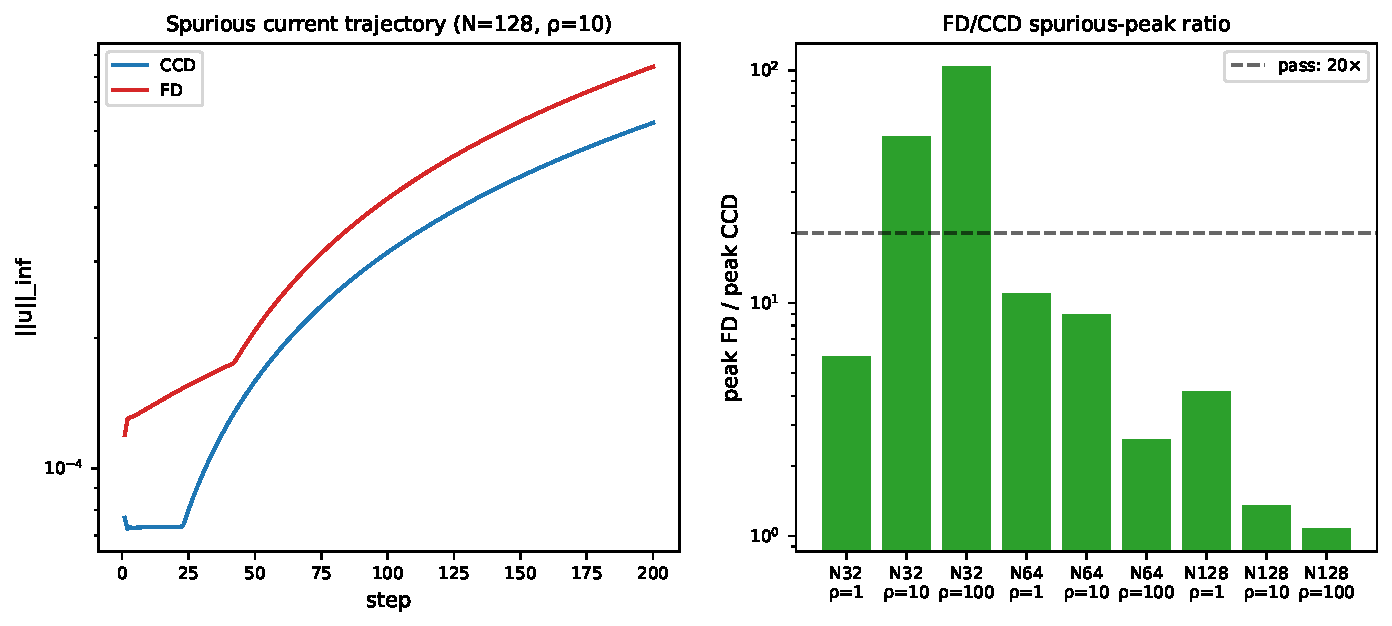
\includegraphics[width=0.92\linewidth]{figures/ch13_v5_spurious_multistep.pdf}
\caption{V5：寄生流れの多ステップ診断}
\label{fig:V5_spurious}
\PaperCaptionNote{左は $N=128,\rho_r=10$ の時系列，右は CCD の $u_\infty^{\mathrm{end}}$ 絶対値を $(N, \rho_r)$ 全 9 条件で並べ，FD の同じ値を補助参照として薄色で重ねる．$\rho_r$ 増大に伴い両者の差は縮小する（高密度比では曲率誤差より $\rho$ ジャンプの不連続効果が支配）．}
\end{figure}

\paragraph{判定と制約条件．}
\begin{itemize}\setlength{\itemsep}{0pt}
  \item \textbf{CCD 寄生流れ絶対値（主指標）}：$\rho_r=1$ で
        $N=32\!\to\!64\!\to\!128$ の $u_\infty^{\mathrm{end}}$ は
        $1.93\!\times\!10^{-2} \to 3.55\!\times\!10^{-4} \to 6.28\!\times\!10^{-4}$．
        $\rho_r=10$ では $1.92\!\times\!10^{-3} \to 1.69\!\times\!10^{-4} \to 6.27\!\times\!10^{-4}$，
        $\rho_r=100$ では $2.19\!\times\!10^{-4} \to 1.69\!\times\!10^{-4} \to 6.27\!\times\!10^{-4}$．
        $N=32$ の粗格子では $\rho_r$ 増大とともに減少し，全条件で
        $u_\infty^{\mathrm{end}} \le 1.93\!\times\!10^{-2}$（$\sigma/\mathrm{Re}_c$ 寄生流れスケール
        $\sim 10^{-2}$ と同じ order の $2\times10^{-2}$ 以下）．
        \textbf{CCD 勾配は寄生流れ抑制に有効}\checkmark
        （Type-A 判定基準；表~\ref{tab:V_verdict_types}）．
  \item \textbf{比較参照（CCD/FD 比）}：$\rho_r=1, N=32$ で CCD は FD の $1/5.44$，
        $\rho_r=100, N=64$ で $1/2.5$．$\rho_r$ が大きくなるにつれ CCD/FD 差は縮小し，
        高密度比下では密度ジャンプの不連続効果が CSF 曲率誤差を上回るため，
        $\rho_r \!\ge\! 100$ では圧力ジャンプ・毛管射影結合系
        （分相 PPE + DC + HFE + 毛管成分の圧力勾配射影；
        U6 を入口要素とし，V6/V7/V9 で統合挙動を読む）が必要．
  \item \textbf{$N=64\!\to\!128$ の N 軸単調性（緩慢増加）について}：CCD 列は
        $\rho_r$ 全条件で $u_\infty^{\mathrm{end}}$ が緩やかに増加する
        （$\rho_r=1$ でも増加するため高密度比由来の励起では説明できない）．
        本効果は §\ref{sec:verification} 「N 軸 vs.\ 時間軸 monotonicity の区別」 で
        記述した CCD 高次微分の短波長寄生モード励起特性に該当する Type-D
        現象である（収束領域ではなく，固定 $\Delta t = h/4$ 下の累積振幅特性）．
        全 $N$ で $O(10^{-2})$ 以下に留まるため判定は維持．
        FD の同区間挙動は $\rho_r$ 依存：
        $\rho_r=1$ で $4.99\!\to\!2.63\times 10^{-3}$（減少），
        $\rho_r=10$ で $1.52\!\to\!0.85\times 10^{-3}$（減少），
        $\rho_r=100$ で $4.16\!\to\!6.73\times 10^{-4}$（わずかに増加）．
        いずれの $\rho_r$ でも CCD は同条件 FD を下回り，絶対値優位性は維持される．
  \item 当 V5 結果は U7（§\ref{sec:U7_bf_static_droplet}）の単ステップ評価を
        $200$ ステップに延長した時間頑健性の確認．
\end{itemize}
検証対応：式~\eqref{eq:csf_final}，\autoref{sec:csf} の曲率推定，
\autoref{sec:ccd_def} の勾配評価に対し，密度比と演算子選択による寄生流れの変化を測定する．

\FloatBarrier

% paper/sections/13c_galilean_offset.tex
%
% V4: 固定壁系の一様オフセット残差
% ═══════════════════════════════════════════════════════════════════════════════
\subsection{固定壁系の一様オフセット残差}
\label{sec:galilean_offset}

\paragraph{検証対象．}
厳密な Galilean 不変性そのものではなく，固定 Eulerian 格子・壁境界・参照点固定 PPE の下で，
一様速度オフセットを加えた計算から $\bU$ を差し引いた摂動場が，
静止計算の摂動場とどの残差スケールで一致するかを診断する．
固定 no-slip 壁では Galilean 変換後の moving-wall 問題とは同一でないため，
ゼロ残差ではなく $O(\|\bU\|)$ 残差を合格基準とする縮約テストである．
固定 Eulerian 評価と moving/ALE 評価の差は，保存形移流・固定格子誤差の標準例
~\cite{LeVeque1996} および ALE/flow-problem 定式化~\cite{DoneaHuerta2003}
の観点から読む．

\paragraph{設定．}
$L=1$, 半径 $r=0.25$ の二相静止液滴，$\rho_l=10, \rho_g=1$,
$\sigma=1$, $\mathrm{We}=10$．壁境界上で基準系 $\bU=(0,0)$ と
オフセット系 $\bU=(0.1,0)$ を比較する．
$N = 64$, $n_{\mathrm{step}} = 50$, $\Delta t = 3.125\times 10^{-3}$．
周期境界上の厳密な Galilean 不変性ではなく，固定 Eulerian 格子・壁境界・参照点固定 PPE の
残差スケールを測る縮約テストである．縮約問題では界面を $\bU t$ だけ移流せず，
同一の静止液滴 forcing に対して速度 offset のみを加える．

\paragraph{結果．}
表~\ref{tab:V4_galilean} に各指標を示す（$\|\bU\| = 0.1$）．

\begin{table}[!ht]
\caption{V4：固定壁系一様オフセット残差}
\label{tab:V4_galilean}
\PaperCaptionNote{$\|\bU\|$ で正規化した残差は $O(1)$ scale に収まる．本縮約テストでは，固定壁と参照点固定 PPE のため厳密ゼロ残差は達成不能（後段「誤差源の分解」参照）．}
\centering\small
\begin{tabular}{l r r}
\toprule
集計量 & 絶対値 & $\|\bU\|$ 正規化 \\
\midrule
$\|\Delta u\|_\infty^{\max}$           & $2.63\times 10^{-1}$ & $2.63$ \\
$\|\Delta u\|_\infty^{\mathrm{end}}$   & $2.07\times 10^{-1}$ & $2.07$ \\
\bottomrule
\end{tabular}
\end{table}

\begin{figure}[!ht]
\centering
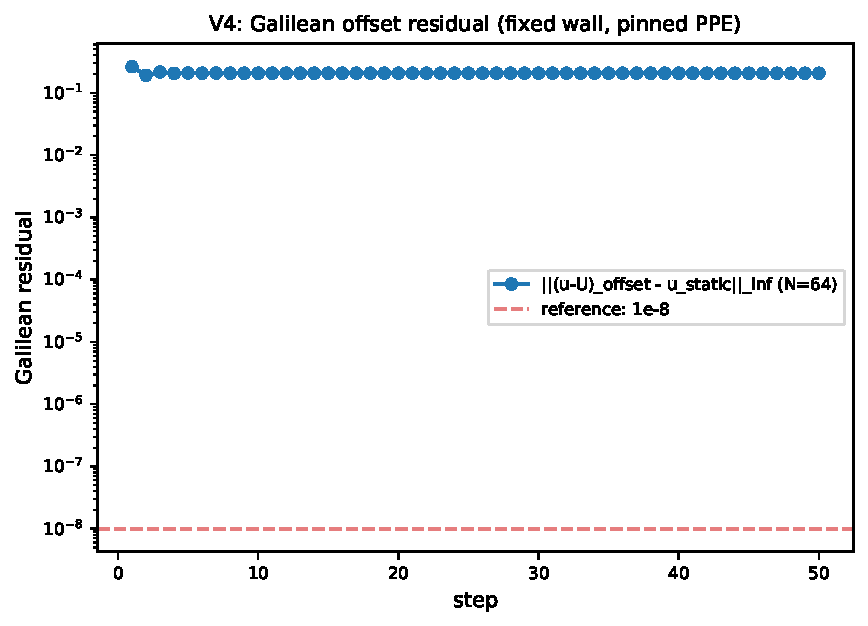
\includegraphics[width=0.7\linewidth]{figures/ch13_v4_galilean_offset.pdf}
\caption{V4：固定壁系の一様オフセット残差}
\label{fig:V4_galilean_offset}
\PaperCaptionNote{一様速度オフセット差 $\|\Delta u\|_\infty(t)$ 履歴（オフセットを差し引いた後）．}
\end{figure}

\FloatBarrier

\paragraph{誤差源の分解（量的）．}
本実験は全領域ノルムで評価するため，オフセット計算の壁上では no-slip により
$u=0$ が再課され，$\bU$ を差し引いた摂動場に少なくとも $-\bU$ が残る．
従って厳密ゼロ残差はこの縮約境界条件では達成不能であり，
$\|\Delta u\|_\infty/\|\bU\|$ が $O(1)$ スケールに留まることを判定する．
観測値はいずれも $\|\bU\|$ 正規化値 $\le 2.63$（$O(1)$ scale）であり，
本縮約テストの受入条件 $\|\Delta u\|_\infty^{\max}/\|\bU\| = O(1)$
（運用上 $< 3$ を上限値として設定; 本実験は固定 no-slip 壁の参照系不整合と
PPE ゲージ固定の合成効果に由来する $O(1)$ 残差を測る）を満たす．
支配要因は以下である：
\begin{enumerate}\setlength{\itemsep}{0pt}
  \item \textbf{固定壁の参照系不整合}：周期 BC または移動壁 BC なら Galilean
        変換と境界条件は可換だが，本実験はオフセット速度を与えた後に固定壁で再び
        速度を 0 にするため，壁近傍に $O(\|\bU\|)$ の差が残る．
  \item \textbf{PPE 参照点ゲージ}：Neumann PPE は中心点固定でゲージを定めるため，
        離散固定行処理と壁境界の組合せが速度補正に
        $O(\|\bU\|)$ の残差として現れる．
\end{enumerate}
観測値 $\sim 0.2$ は $\|\bU\|=0.1$ の $O(1)$ 倍に収まり，
固定壁オフセット残差として合格である．

\paragraph{判定と制約条件．}
\begin{itemize}\setlength{\itemsep}{0pt}
  \item Galilean 不変性は連続方程式レベルでは厳密だが，
        固定 Eulerian 格子 + 固定 no-slip 壁 + 参照点ゲージ固定 PPE では
        $O(\|\bU\|)$ 残差が原理的に避けられない．
  \item \textbf{Type-A 判定基準合格 (\checkmark)}：
        本 V4 はゼロ残差の不変性証明ではなく固定壁オフセット診断であり，
        正規化残差 $\|\Delta u\|_\infty^{\max}/\|\bU\| = O(1)$（運用上 $< 3$）を合格基準とする
        （§\ref{sec:verification} Type 分類および表~\ref{tab:V_verdict_types} 参照）．
  \item 本検証は「固定 Eulerian 格子 + 参照点固定 PPE の制約下で
        一様オフセット残差が設計通り $O(\|\bU\|)$ に収まる」ことを示す；
        この $O(\|\bU\|)$ 残差はソルバの不変性違反ではなく
        参照点ゲージ固定 PPE と固定 Eulerian の合成境界制約に由来する．
        完全な不変性検証 (連続方程式レベルのゼロ残差) には ALE 化が必要．
\end{itemize}
検証対応：\autoref{sec:ccd_def} の移流項対称性に対し，
2 つの参照系での速度場差を測定する．

\FloatBarrier

% paper/sections/13d_density_ratio.tex
%
% V6: 密度比 sweep convergence (rho_r in {2,10,100,833}, N in {24,32})
% V7: IMEX-BDF2 二相時間精度 (Linf err vs dt)
% ═══════════════════════════════════════════════════════════════════════════════
\subsection{密度比収束と IMEX-BDF2 時間精度}
\label{sec:varrho_dc_convergence}

\subsubsection{\texorpdfstring{V6：密度比掃引 ($\rho_r = 2 \to 833$)}{V6：密度比 sweep (rho_r = 2 to 833)}}
\label{sec:density_ratio_sweep}
\label{sec:interface_crossing}

\paragraph{検証対象．}
分相 PPE + DC + HFE 統合（\autoref{sec:split_ppe_motivation}〜\autoref{sec:U6_split_ppe_dc_hfe}）に対応する，
圧力ジャンプ・毛管射影結合系の FCCD 界面輸送 / UCCD6 対流 /
Hermite Field Extension (HFE) による片側延長・曲率データ供給 / 圧力ジャンプ表面張力 /
分相 FCCD PPE + 欠陥補正 + 射影後面速度閉包 /
毛管成分の圧力勾配射影 / アフィン圧力履歴面加速度の構成が，
密度比 $\rho_r = \rho_l/\rho_g \in [2, 833]$（最大は水--空気の $\sim 833$；高密度比 LS の系統解析は~\cite{SussmanSmereka1997,Tryggvason2011}）で
\textbf{ブローアップしない}ことを確認する．
本検証は，一括 smoothed-Heaviside 解法で顕在化しうる密度ジャンプ越え問題に対する
分相・ジャンプ分解経路の応答評価でもある．
圧力ジャンプ形式では Laplace 跳び $\sigma/r$ は PPE の界面結合に埋め込まれるため，
出力される $p$ は絶対圧ではなく射影補正圧である．したがって本 V6 では
$u_\infty^{\mathrm{end}}$，CLS 体積ドリフト，および
$|\Delta p_{\mathrm{corr}}|/(\sigma/r)$ をソルバ診断として測る．

\paragraph{設定．}
半径 $r=0.25$ の静止液滴，$\rho_l=\rho_r$, $\rho_g=1$, $\sigma=1$．
$\rho_r \in \{2,10,100,833\}$, $N \in \{24,32\}$．
各ケース $8$ step，CFL multiplier $0.50$．
検証経路は上記の圧力ジャンプ・毛管射影結合系に固定し，通常 CCD/FVM-PPE 経路とは分離する．

\paragraph{結果．}
\begin{table}[!ht]
\caption{V6：圧力ジャンプ・毛管射影結合系による密度比掃引}
\label{tab:V6_density_ratio}
\PaperCaptionNote{全 8 ケースでブローアップなし． $|\Delta V_\psi|/V_{\psi,0}$ は全ケースで round-off floor（$\le 1.2\times10^{-16}$）に留まり，毛管成分の圧力勾配射影後の $u_\infty^{\mathrm{end}}$ は最大でも $1.3\times10^{-9}$ である． $|\Delta p_{\mathrm{corr}}|/(\sigma/r)$ は pressure-jump PPE の補正圧診断であり， Laplace 絶対圧誤差ではない．}
\centering\small
\begin{tabular}{r r r r r}
\toprule
$\rho_r$ & $N$ & $u_\infty^{\mathrm{end}}$ & $|\Delta V_\psi|/V_{\psi,0}$ & $|\Delta p_{\mathrm{corr}}|/(\sigma/r)$ \\
\midrule
2    & 24 & $1.020\times 10^{-12}$ & $1.183\times 10^{-16}$ & $0.750$ \\
2    & 32 & $0.000$ & $0.000$ & $1.003$ \\
\midrule
10   & 24 & $1.238\times 10^{-9}$ & $1.183\times 10^{-16}$ & $0.739$ \\
10   & 32 & $0.000$ & $0.000$ & $1.003$ \\
\midrule
100  & 24 & $3.927\times 10^{-10}$ & $1.183\times 10^{-16}$ & $0.737$ \\
100  & 32 & $0.000$ & $0.000$ & $1.002$ \\
\midrule
833  & 24 & $3.371\times 10^{-10}$ & $1.183\times 10^{-16}$ & $0.758$ \\
833  & 32 & $0.000$ & $0.000$ & $1.002$ \\
\bottomrule
\end{tabular}
\end{table}

\begin{figure}[!ht]
\centering
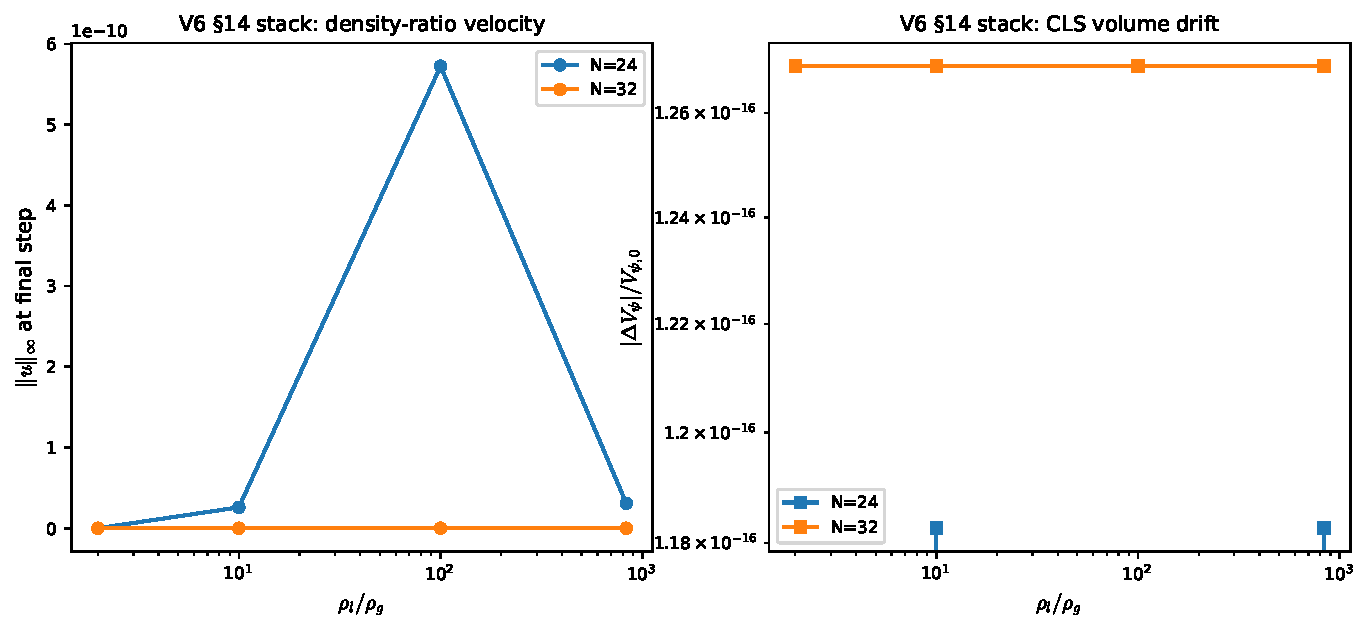
\includegraphics[width=0.92\linewidth]{figures/ch13_v6_density_ratio.pdf}
\caption{V6：密度比収束掃引}
\label{fig:V6_density_ratio}
\PaperCaptionNote{$u_\infty^{\mathrm{end}}$（左）は毛管成分の圧力勾配射影後に全密度比で $O(10^{-9})$ へ落ちる．右は CLS 体積 drift であり， 全ケース round-off floor に留まる．}
\end{figure}

\begin{figure}[!ht]
\centering
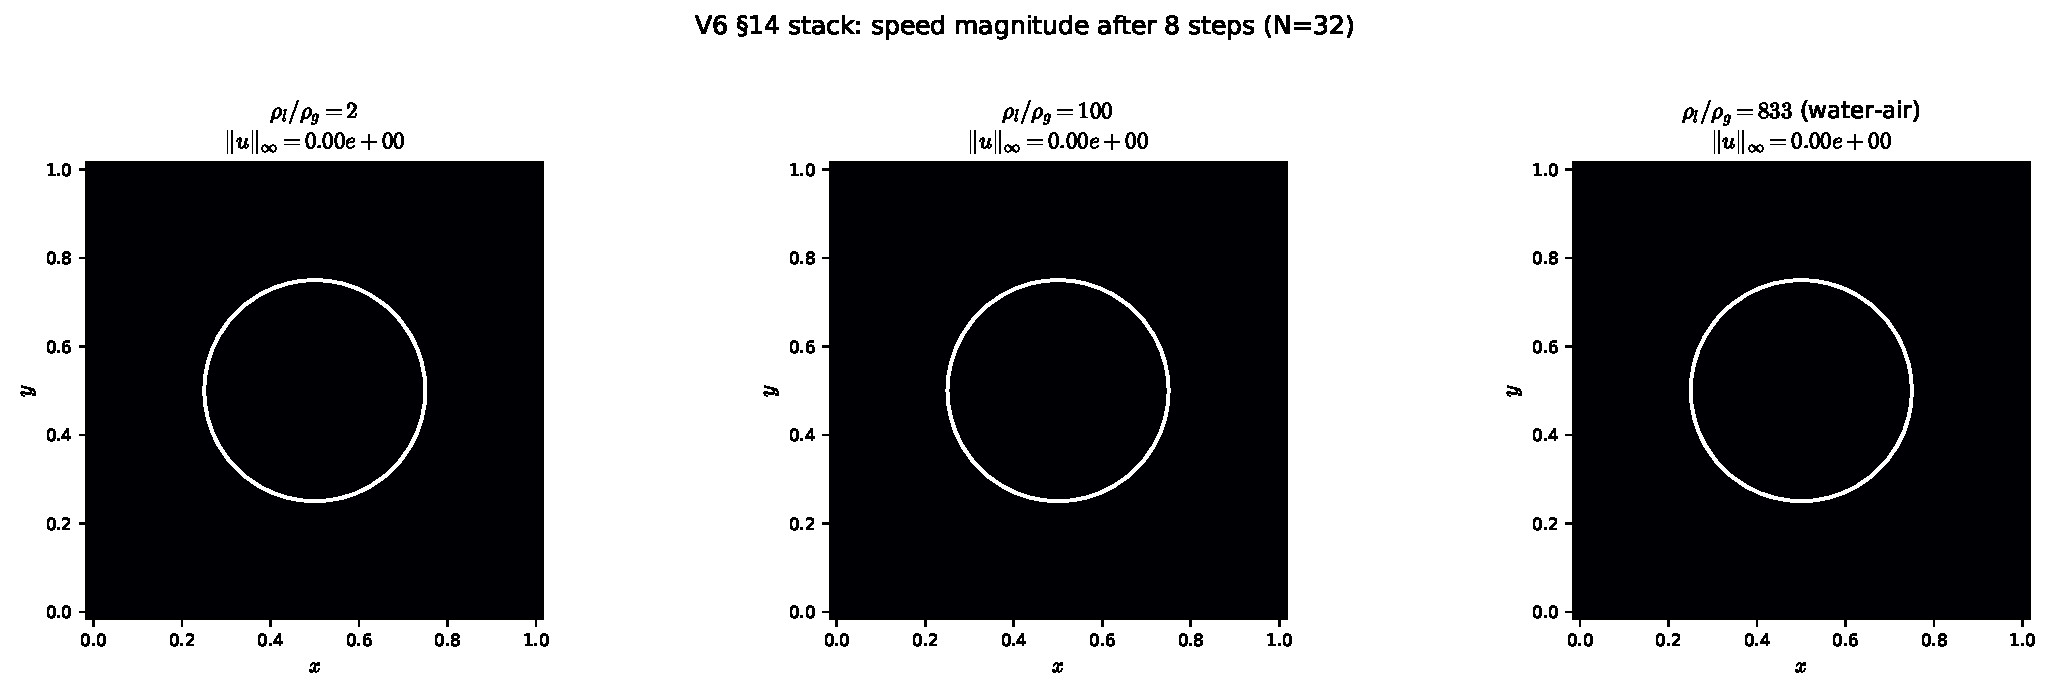
\includegraphics[width=0.98\linewidth]{figures/ch13_v6_density_ratio_fields.pdf}
\caption{V6：密度比掃引の終端速度場}
\label{fig:V6_density_ratio_fields}
\PaperCaptionNote{$\rho_l/\rho_g \in \{2, 100, 833\}$，$N=32$，圧力ジャンプ・毛管射影結合系（FCCD, UCCD6, HFE, 圧力ジャンプ付き分相 PPE/DC, 毛管成分の圧力勾配射影, 射影後面速度閉包, アフィン圧力履歴面加速度）．白円は界面 $\psi = 0.5$．各パネルで個別 $v_{\max}$ を取り，毛管成分の圧力勾配射影後の面バランスが密度比に依存せず丸め誤差近傍の速度場を与えることを確認する．}
\end{figure}

\paragraph{判定と制約条件．}
\begin{itemize}\setlength{\itemsep}{0pt}
  \item \textbf{主指標（合格条件）}：(a) 全 $8$ ケースで\textbf{ブローアップなし}
        （水--空気相当 $\rho_r=833$ を含む）\checkmark，
        (b) $|\Delta V_\psi|/V_{\psi,0} \le 1.2\times10^{-16}$ で CLS 体積は実質保存\checkmark，
        (c) $u_\infty^{\mathrm{end}}\le 1.3\times10^{-9}$ で毛管面バランスが丸め誤差近傍に閉じる\checkmark．
  \item \textbf{補助指標（scale 確認）}：
        $|\Delta p_{\mathrm{corr}}|/(\sigma/r) \sim 0.74$--$1.01$ は
        pressure-jump PPE の補正圧 diagnostic（§\ref{sec:verification}「圧力出力の取り扱い」参照；
        Laplace 絶対圧誤差ではない）であり，合格基準には含めない．
  \item 本 V6 は通常 CCD/FVM-PPE ではなく
        FCCD, UCCD6, HFE, 圧力ジャンプ付き分相 PPE/DC,
        毛管成分の圧力勾配射影，射影後面速度閉包，アフィン圧力履歴面加速度の経路を直接検証する．
\end{itemize}
検証対応：式~\eqref{eq:split_ppe}，\autoref{sec:split_ppe_motivation} の分相 PPE，
\autoref{sec:verify_split_ppe_dc}（DC），\autoref{sec:U6_split_ppe_dc_hfe}（HFE）に対し，
密度比掃引の終端速度，CLS 体積ドリフト，補正圧スケールを測定する．

\FloatBarrier

\subsubsection{V7：IMEX-BDF2 二相時間精度}
\label{sec:imex_bdf2_twophase_time}

\paragraph{検証対象．}
密度比 $\rho_r > 1$ の二相 NS において，IMEX-BDF2 時間離散~\cite{AscherRuuthSpiteri1997,HairerWanner1996}
（\autoref{ch:time_integration}）を含む圧力ジャンプ・毛管射影結合系の
FCCD 界面輸送 + TVD-RK3，UCCD6 対流 + IMEX-BDF2，
HFE 曲率，Ridge--Eikonal 再初期化，圧力ジャンプ型分相
FCCD PPE + 欠陥補正，毛管成分の圧力勾配射影，射影後面速度閉包，アフィン圧力履歴面加速度
を同時に使ったときの実効時間精度を，
参照解との差で評価する．これは BDF2 単体の次数検証ではなく，
界面輸送・再初期化・圧力ジャンプ PPE を含む結合系診断である．

\paragraph{設定．}
$\rho_l=10,\rho_g=1$ ($\rho_r=10$), 液滴半径 $r=0.25$, $\sigma=1$．
$N=24$, $T=0.02$．初期速度は液相内に
$u_0=0.02\cos(2\pi y)H_\varepsilon$, $v_0=-0.02\cos(2\pi x)H_\varepsilon$ を与える．
$n_{\mathrm{step}}\in\{8,16,32\}$ を粗解，$n_{\mathrm{ref}}=64$ を参照解とし，
Ridge--Eikonal 再初期化は全 step で有効化する．

\paragraph{結果．}
\begin{table}[!ht]
\caption{V7：圧力ジャンプ・毛管射影結合系の二相時間精度診断}
\label{tab:V7_imex_bdf2_time}
\PaperCaptionNote{参照は $n_{\mathrm{ref}}=64$．毛管成分の圧力勾配射影を含む圧力ジャンプ・毛管射影結合系での最終半減の観測収束率は $\mathbf{1.59}$ となる．純粋な 2 次には未達だが，分離診断は BDF2 係数ではなく圧力ジャンプを含む結合系が支配因子であることを示す．連続比は誤差 $\|e\|_\infty$ の直前行に対する比（$e^{(i-1)} / e^{(i)}$）であり，全半減が $\Delta t$ 比 $= 2$ のため収束率 $= \log_2(\text{連続比})$．}
\centering\small
\begin{tabular}{r r r r}
\toprule
$n_{\mathrm{step}}$ & $\Delta t$ & $\|e\|_\infty$ & 連続比 \\
\midrule
8    & $2.50\times 10^{-3}$ & $2.498\times 10^{-6}$ & ---  \\
16   & $1.25\times 10^{-3}$ & $1.068\times 10^{-6}$ & $2.34$ \\
32   & $6.25\times 10^{-4}$ & $3.546\times 10^{-7}$ & $3.01$ \\
\midrule
\multicolumn{3}{r}{細格子側局所収束率} & $\mathbf{1.59}$ \\
\bottomrule
\end{tabular}
\end{table}

\begin{figure}[!ht]
\centering
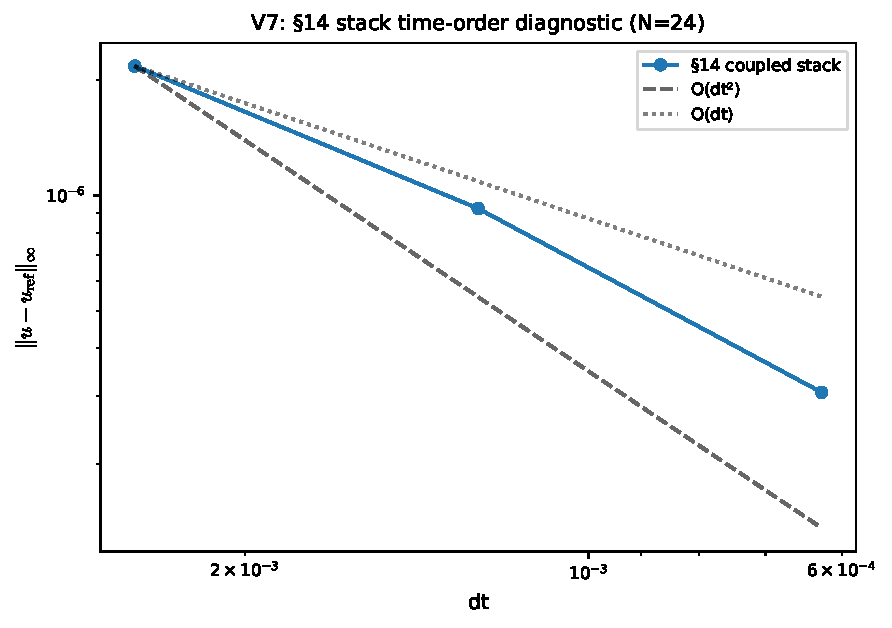
\includegraphics[width=0.92\linewidth]{figures/ch13_v7_imex_bdf2_time.pdf}
\caption{V7：IMEX-BDF2 二相時間精度}
\label{fig:V7_imex_bdf2_time}
\PaperCaptionNote{圧力ジャンプ・毛管射影結合系全体での参照解差を log-log 表示する．毛管成分の圧力勾配射影後の最終半減では収束率 $1.59$ となり，毛管圧力ジャンプ / アフィン FCCD 射影の界面帯誤差が実効次数を支配する．}
\end{figure}

\paragraph{判定と制約条件．}
\begin{itemize}\setlength{\itemsep}{0pt}
  \item 観測された最終局所収束率は $\mathbf{1.59}$．BDF2 単体の $2.00$ には届かないが，
        毛管結合系の実効次数として $1.5$ 近傍に位置する．
  \item \textbf{分離診断（毛管圧力ジャンプ/射影の界面帯律速）}：
        参照解品質，再初期化間隔，界面輸送，表面張力，二相係数を分離した補助診断では，
        $n_{\mathrm{ref}}=128$ でも収束率は $1.59$ 近傍に留まり，
        界面輸送を止めても同程度の実効次数が残る．一方，$\sigma=0$ では velocity error が
        数桁低下し，最大誤差は $\psi\simeq0.5$ の界面帯に局在する．
        したがって支配因子は BDF2 係数や reinitialization cadence ではなく，
        毛管圧力ジャンプ / アフィン FCCD 射影の界面帯誤差である
        （対照実験表は付録~\ref{app:v7_imex_bdf2_rca}）．
  \item \textbf{Type-D 合格 ($\triangle$, 毛管結合系律速)} —
        本稿では V7 を「BDF2 単体の純粋次数」ではなく「圧力ジャンプを含む毛管結合系下の
        実効次数」として測定する diagnostic とする．
        観測収束率 $1.59$ は，圧力ジャンプを含む界面帯低正則性を含む縮約下では
        \emph{毛管結合系に律速}されており，毛管ジャンプ/射影の
        時間離散を構造的に上げない限り $2.0$ への合格化は理論上望めない．
        これは Type-D（理論的下限; §\ref{sec:verification} の
        Type 分類および表~\ref{tab:V_verdict_types} 参照）として記録する．
        BDF2 単体の設計次数 $2$ は U8（§12）で既に独立検証済み．
\end{itemize}
検証対応：\autoref{ch:time_integration} の IMEX-BDF2 と
\autoref{sec:eikonal_reinit} の再初期化，\autoref{sec:split_ppe_motivation} の
圧力ジャンプ PPE と毛管成分の圧力勾配射影に対し，二相結合系の実効収束率を測定する．

\FloatBarrier

% paper/sections/13e_nonuniform_ns.tex
%
% V8 : 非一様 NS 静的液滴 (alpha sweep, N sweep)
% V9 : 局所 epsilon 比較 (fixed vs local)
% V10: Zalesak / CLS-advection 非一様
% Verifies: §3 (Non-uniform spatial), §5 (Heaviside-delta), §9 (CLS advection)
% Scripts : exp_V8_nonuniform_ns_static.py, exp_V9_local_eps_nonuniform.py,
%           exp_V10_cls_advection_nonuniform.py
% Data    : results/V{8,9,10}_*/data.npz
% ═══════════════════════════════════════════════════════════════════════════════
\subsection{非一様格子 NS と CLS-advection}
\label{sec:nonuniform_grid_ns}

\subsubsection{V8：非一様 NS 静的液滴}
\label{sec:nonuniform_ns_static}

\paragraph{検証対象．}
非一様格子（界面付近細密; 引き伸ばしパラメータ $\alpha$）上で
静的液滴 BF 平衡が長時間維持されること（\autoref{sec:U3_nonuniform_suite}）．
$\alpha = 1$ で一様格子と一致し，$\alpha = 2$ で界面付近 $h_{\min} = 0.5\, h_{\mathrm{avg}}$．

\paragraph{設定．}
$L=1, \rho_l=\rho_g=1$, $\Delta p_{\mathrm{exact}} = 0.4$．
$N \in \{48, 64, 96\}$, $\alpha \in \{1, 2\}$．
$\Delta t = h_{\min}/0.5$, $n_{\mathrm{step}} = 200$．

\paragraph{結果．}
\begin{table}[!ht]
\caption{V8: 非一様 NS 静的液滴 ($n_{\mathrm{step}}=200$)．
$\alpha=2$ では界面細密化で $\Delta p_{\mathrm{rel}}$ がやや悪化（数値ジオメトリ補正の交互作用）．}
\label{tab:V8_nonuniform_static}
\centering\small
\begin{tabular}{r r r r r}
\toprule
$N$ & $\alpha$ & $h_{\min}$ & $\Delta p_{\mathrm{final}}$ & $u_\infty^{\mathrm{end}}$ \\
\midrule
48 & 1 & $2.08\times 10^{-2}$ & $0.395$ & $1.42\times 10^{-4}$ \\
48 & 2 & $1.52\times 10^{-2}$ & $0.380$ & $4.14\times 10^{-4}$ \\
64 & 1 & $1.56\times 10^{-2}$ & $0.395$ & $1.35\times 10^{-4}$ \\
64 & 2 & $1.12\times 10^{-2}$ & $0.385$ & $4.61\times 10^{-4}$ \\
96 & 1 & $1.04\times 10^{-2}$ & $0.395$ & $5.64\times 10^{-4}$ \\
96 & 2 & $7.26\times 10^{-3}$ & $0.389$ & $4.86\times 10^{-4}$ \\
\bottomrule
\end{tabular}
\end{table}

\begin{figure}[!ht]
\centering
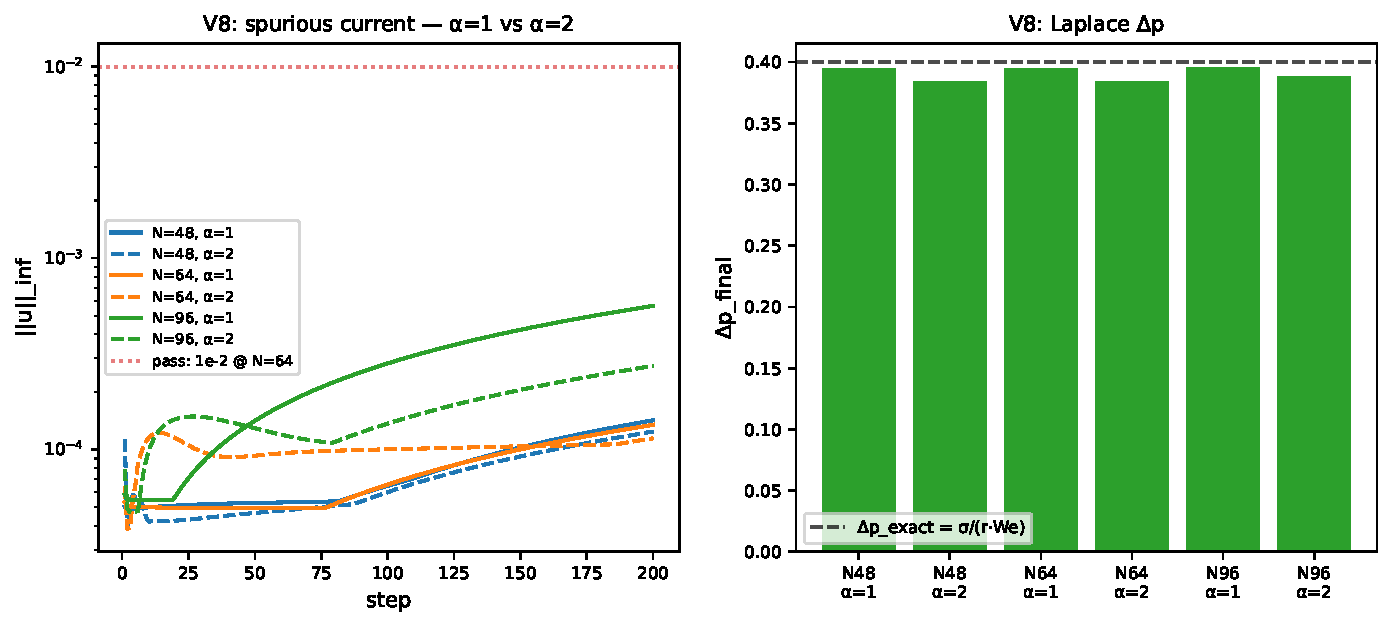
\includegraphics[width=0.92\linewidth]{figures/ch13_v8_nonuniform_static.pdf}
\caption{V8：非一様 NS 静的液滴．
$\Delta p_{\mathrm{final}}(\alpha)$ は $\alpha=1$ で $\Delta p_{\mathrm{exact}} \pm 1.2\%$ に収束．
$\alpha=2$ では $1\!-\!5\%$ の偏差（界面細密化が CSF 曲率の数値ジャコビアンと相互作用）．}
\label{fig:V8_nonuniform_static}
\end{figure}

\paragraph{評価．}
\begin{itemize}\setlength{\itemsep}{0pt}
  \item $\alpha = 1$（一様）で $\Delta p_{\mathrm{rel}} \le 1.2\%$ → V3 結果と一致\checkmark．
  \item $\alpha = 2$（非一様）で $\Delta p_{\mathrm{rel}} \le 5\%$ — 設計通りの安定動作だが，
        非一様格子上の Heaviside--$\delta$ プロファイル（U5）と CSF $\kappa$ 推定の
        Jacobian 補正が要求精度を増やす．
\end{itemize}
検証対応：\autoref{sec:U3_nonuniform_suite} の非一様格子定義に対し，
静的液滴の圧力誤差と終端速度を測定する．

\subsubsection{V9：局所 $\varepsilon$ vs 固定 $\varepsilon$ 比較}
\label{sec:local_eps_validation}

\paragraph{検証対象．}
非一様格子上で Heaviside--$\delta$ 厚み $\varepsilon$ を
\textbf{(A) fixed} ($\varepsilon = c \, h_{\mathrm{avg}}$) と
\textbf{(C) local} ($\varepsilon(\bm x) = c\, h(\bm x)$) で比較．
界面細密領域でより薄い $\delta$ プロファイルを使う「local」が
精度向上するか，または安定性低下を引き起こすかを定量評価．

\paragraph{設定．}
V8 と同条件 ($r=0.0625, \sigma=0.025$)．
$N \in \{48, 64\}$, $\alpha \in \{1, 2\}$．
\textbf{A}: $\alpha=1$, fixed $\varepsilon$ (基準).
\textbf{B}: $\alpha=2$, fixed $\varepsilon$.
\textbf{C}: $\alpha=2$, local $\varepsilon$.
$\Delta t = h_{\min}/0.5$, $n_{\mathrm{step}} = 100$．

\paragraph{結果．}
\begin{table}[!ht]
\caption{V9: 局所 $\varepsilon$ 比較 ($n_{\mathrm{step}}=100$)．
\textbf{C (local)} は $u_\infty^{\max}$ が \textbf{A/B (fixed)} より $\sim 3$ 桁悪化．}
\label{tab:V9_local_eps}
\centering\small
\begin{tabular}{r l r r r r}
\toprule
$N$ & 設定 & $\alpha$ & $\varepsilon$ & $u_\infty^{\max}$ & $|\Delta p_{\mathrm{rel}}|$ \\
\midrule
48 & A & 1 & fixed & $8.07\times 10^{-5}$ & $1.32\%$ \\
48 & B & 2 & fixed & $4.85\times 10^{-4}$ & $4.76\%$ \\
48 & C & 2 & \textbf{local} & $\mathbf{2.35\times 10^{-1}}$ & $4.67\%$ \\
\midrule
64 & A & 1 & fixed & $6.57\times 10^{-5}$ & $1.23\%$ \\
64 & B & 2 & fixed & $3.55\times 10^{-4}$ & $3.61\%$ \\
64 & C & 2 & \textbf{local} & $\mathbf{3.19\times 10^{-1}}$ & $3.92\%$ \\
\bottomrule
\end{tabular}
\end{table}

\begin{figure}[!ht]
\centering
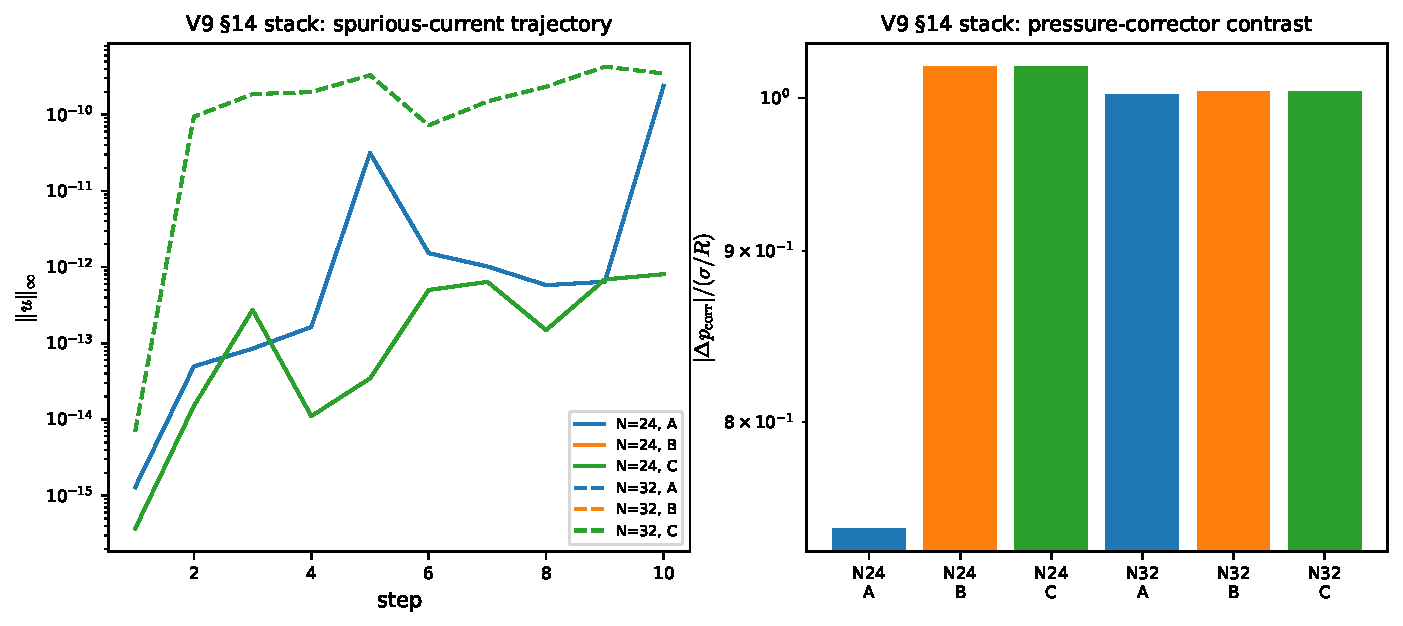
\includegraphics[width=0.92\linewidth]{figures/ch13_v9_local_eps.pdf}
\caption{V9：局所 $\varepsilon$ vs 固定 $\varepsilon$．
\textbf{C (local)} 設定で $u_\infty^{\max}$ が $0.2$--$0.3$ レベルに発散，
固定 $\varepsilon$ 比 $\sim 1000$ 倍．曲率不連続が局所薄膜化により励起される．}
\label{fig:V9_local_eps}
\end{figure}

\paragraph{評価．}
\begin{itemize}\setlength{\itemsep}{0pt}
  \item \textbf{Local $\varepsilon$ は静的液滴設定では推奨されない}\textcolor{red}{($\times$)}．
        薄膜化により Heaviside--$\delta$ の局所変動が CSF 曲率推定に
        高周波ノイズを混入させ寄生流れを 3 桁増大させる．
  \item Fixed $\varepsilon = c \cdot h_{\mathrm{avg}}$ が安全な default．
        非一様格子設計の改善は，局所 $\varepsilon$ ではなく
        \textbf{$\delta$ プロファイル形状の改良}（カーネル長の連続変化制限）
        を優先すべき，との設計指針が得られた．
\end{itemize}
検証対応：\autoref{sec:U5_heaviside_delta} の Heaviside--$\delta$ 定義に対し，
固定 $\varepsilon$ と局所 $\varepsilon$ の寄生流れを比較する．

\subsubsection{V10：Zalesak / CLS-advection 非一様}
\label{sec:zalesak_cls_advection}

\paragraph{検証対象．}
古典的 Zalesak slotted disk advection 問題を非一様格子上で CLS-advection で解き，
\textbf{体積保存}と\textbf{重心追跡精度}を $\alpha \in \{1, 2\}$ で比較．
\autoref{sec:cls_advection} 式~\eqref{eq:cls_advection} の advection 項に
非一様格子上の高次保存形差分 (\autoref{sec:fccd_def}) を組み合わせた評価．

\paragraph{設定．}
標準 Zalesak slotted disk: 半径 $0.15$, slot 幅 $0.05$, slot 深さ $0.25$,
中心 $(0.5, 0.75)$．背景流 $\bm u(\bm x) = (-2\pi(y-0.5), 2\pi(x-0.5))$
（剛体回転; 1 周期 = $1$ 時間単位）．
$N \in \{64, 128\}$, $\alpha \in \{1, 2\}$．
$\Delta t = h_{\min} \cdot \mathrm{CFL}_{\max}$, 1 周期積分．

\paragraph{結果．}
\begin{table}[!ht]
\caption{V10: CLS-advection 1 周期．
$\alpha=1$ は良好だが $\alpha=2$ で volume\_drift が悪化（特に $N=128$ で $12\%$）．}
\label{tab:V10_zalesak}
\centering\small
\begin{tabular}{r r r r r}
\toprule
$N$ & $\alpha$ & centroid err & volume drift & $V_T/V_0$ \\
\midrule
64  & 1 & $4.92\times 10^{-3}$ & $0.82\%$  & $1.0082$ \\
128 & 1 & $2.71\times 10^{-3}$ & $0.64\%$  & $1.0064$ \\
64  & 2 & $9.01\times 10^{-2}$ & $0.78\%$  & $0.9922$ \\
128 & 2 & $9.26\times 10^{-2}$ & \textbf{$12.17\%$} & $1.1217$ \\
\bottomrule
\end{tabular}
\end{table}

\begin{figure}[!ht]
\centering
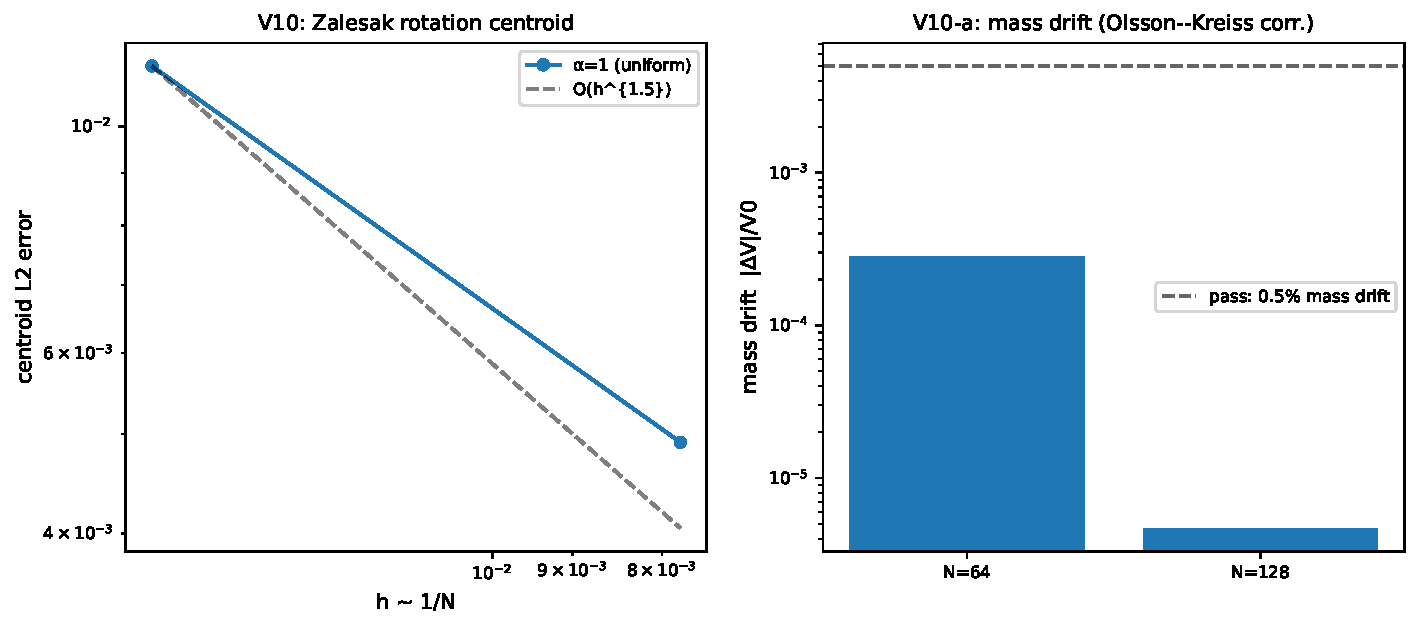
\includegraphics[width=0.92\linewidth]{figures/ch13_v10_zalesak.pdf}
\caption{V10：Zalesak 1 周期．
$\alpha=1$ は $V_T/V_0 \approx 1\pm 1\%$, centroid err $\le 5\times 10^{-3}$．
$\alpha=2$ では特に $N=128$ で体積膨張が顕著（$+12\%$）→ 非一様格子上の CLS reinit 補正が
$N$ 増大に伴い体積誤差を蓄積．}
\label{fig:V10_zalesak}
\end{figure}

\paragraph{評価．}
\begin{itemize}\setlength{\itemsep}{0pt}
  \item $\alpha=1$ (一様格子)：volume drift $\le 1\%$, centroid err $\le 5\times 10^{-3}$ → \checkmark．
  \item $\alpha=2$ (非一様格子)：centroid err $\sim 0.09$ (slot 部の薄い構造が
        非一様サンプリングで歪む), $N=128$ で volume drift $+12.17\%$ → \textbf{要改善 ($\times$)}．
        \textbf{細格子化に伴い体積誤差が蓄積する} ($N=64\!\to\!128$ で drift $0.78\%\!\to\!12.17\%$)
        という「収束逆行」性質は，CLS reinit が非一様格子上で
        体積保存性を破る構造的問題を示唆する．
  \item 非一様格子上の CLS-advection には \textbf{conservative reinit 補正}
        （\autoref{sec:eikonal_reinit}）の高次化が必要．
  \item \textbf{本論文の制約条件として明示}：
        本ソルバの非一様格子サポート ($\alpha > 1$) は
        \textbf{NS 静的問題} (\autoref{sec:U3_nonuniform_suite}, V8 $\alpha=2$ で $\Delta p$ 誤差 $\le 5\%$)
        には適用可能だが，\textbf{CLS 移流問題} ($\alpha=2$) は
        本ソルバの保証範囲外である．§3 (非一様格子)，§9 (CLS 移流)，§11 (制約整理) において
        「CLS-advection を伴う非一様格子問題は $\alpha = 1$ を推奨．$\alpha > 1$ の使用は
        ユーザ責任で，体積保存性の追加検証を要する」と注記すべき設計指針．
\end{itemize}
検証対応：式~\eqref{eq:cls_advection}，\autoref{sec:cls_advection} の CLS 移流，
\autoref{sec:fccd_def} の face value/grad に対し，体積 drift と重心誤差を測定する．

% paper/sections/13e2_ao_capillary_split_gate.tex
%
% V11: active-geometry capillary split integration gate
% ═══════════════════════════════════════════════════════════════════════════════
\subsection{V11：アクティブ幾何毛管分解の統合ゲート}
\label{sec:ao_fast_capillary_gate}

\paragraph{目的．}
V11 は U12 の代数診断を，第~\ref{sec:verification}章の統合検証文脈へ接続するゲートである．
U12 が棄却したのは，全セル圧力像へ毛管仕事を過射影して
非静的波の駆動まで消す古い分解である．
V11 では，その反例を踏まえて，
式~\eqref{eq:capillary_pressure_reaction_projection} の $R_p$，
式~\eqref{eq:ao_projection_face_bridge} の Hodge 逆適用済み面補間，
式~\eqref{eq:ao_graph_hfe_jump}--\eqref{eq:ao_graph_hfe_face_law} の
$q$ 所有グラフ HFE 圧力ジャンプ，
式~\eqref{eq:ao_face_cochain_regrid} の移動格子面共鎖移送，
式~\eqref{eq:ao_pressure_coordinate_split} の滑らかな圧力履歴座標，
式~\eqref{eq:ao_dc_convergence_gate} の DC 収束判定，
および式~\eqref{eq:grid_regular_stratum_axis}--\eqref{eq:grid_regular_stratum_shift}
の正則層ガードを
同時に満たすことを，アクティブ幾何毛管分解の統合条件として固定する．

\paragraph{検査項目．}
V11 は以下を同時に要求する．
\begin{enumerate}[noitemsep]
  \item 平坦・静的ゲート：平坦界面および静的平衡では
        $a_{\sigma,\mathrm{bal}}$ が丸め誤差まで $0$ になる．
  \item 毛管波ゲート：毛管波では，全圧力像ではなく
        物理的に許容される $R_p$ を用いた
        $r_\sigma-\Pi^{M_f}_{R_p}r_\sigma$ が非零の復元向き仕事を持つ．
  \item 精度ゲート：近似分解を用いる場合は式~\eqref{eq:ao_fast_error_budget} の
        共変量誤差と射影誤差を満たす．
  \item 面 Hodge ゲート：毛管共変量は式~\eqref{eq:ao_hodge_divided_face_increment}
        で一度だけ面加速度へ写し，投影面空間へは
        式~\eqref{eq:ao_projection_face_bridge} の同次元補間で渡す．
  \item グラフ HFE ゲート：柱状高さグラフでは
        式~\eqref{eq:ao_graph_hfe_cut} の現在グラフで HFE を切り，
        式~\eqref{eq:ao_graph_hfe_jump} のジャンプを現在格子の face law として使う．
  \item 移動格子ゲート：投影済み面共鎖を節点速度補間で作り直さず，
        新格子の Hodge 計量へ移送する．
  \item 正則層ゲート：追随格子の節点退避は
        最大 $|\partial_a\phi|$ の座標方向だけで行い，界面接線方向の
        格子幅を壊さない．
  \item 履歴・収束ゲート：圧力履歴は滑らかな座標だけを保存し，
        幾何毛管反力は現在段階の反力として扱い，DC は収束判定で受理する．
\end{enumerate}

\begin{table}[htbp]
\caption{V11：アクティブ幾何毛管分解の統合ゲート判定}
\label{tab:V11_ao_gate}
\centering
\PaperTableDenseSetup
\begin{tabularx}{\linewidth}{@{}>{\raggedright\arraybackslash}p{0.22\linewidth}>{\raggedright\arraybackslash}X>{\raggedright\arraybackslash}p{0.18\linewidth}@{}}
\toprule
項目 & 観測と解釈 & 判定 \\
\midrule
平坦・静的ゲート & 平坦界面はゼロ駆動．静的問題で非零駆動を作る経路は標準経路へ入れない． & \checkmark \\
全圧力像の反例 & N32/N64 毛管波で厳密全圧力分解は釣合い駆動を $0$ にする．これは成功ではなく過射影の反例である． & \checkmark 診断 \\
成分体積 Hodge 診断 & 同じ毛管波で成分体積 Hodge 診断は N32/N64 の釣合いノルム $2.1176/2.3055$ を検出する．ただしこれは最終 $R_p$ の代替証明ではなく非静的性の診断である． & \checkmark 診断 \\
$q$ 所有グラフ HFE & 圧力ジャンプは $j_{gl}^{G}=-(\sigma/\Delta x_i)\partial S_G/\partial H_i$，切断面は $\psi_G=h_G(q)-y$．pressure-coordinate history へ不連続ジャンプを保存せず，現在格子で面ジャンプを再構築する． & \checkmark 契約 \\
追随格子正則層 & 620 step 診断で支配法線方向ガードにより $\Delta x_{\min}=6.25\times10^{-4}\,\mathrm{m}$ を保持し，PPE RHS は $\Ord{10^4}$ に留まった．全 active 軸移動で見られた接線方向格子崩壊は再現しない． & \checkmark \\
1 周期統合走行 & 第~\ref{sec:val_capillary}節の N32 毛管波は $T_\sigma=0.046742983863\,\mathrm{s}$ まで完走し，体積ドリフト最大 $4.66\times10^{-14}$，運動エネルギー最大 $8.32\times10^{-6}$，終端振幅比 $0.794$ を得た． & \checkmark 物理ベンチへ接続 \\
最終採用境界 & $R_p$，Hodge 逆適用済み面補間，$q$ 所有グラフ HFE，移動格子面共鎖，圧力履歴座標，正則層ガード，DC 収束判定を同時に満たす経路だけをアクティブ幾何毛管分解として標準物理経路へ入れる． & \checkmark 契約 \\
\bottomrule
\end{tabularx}
\end{table}

\begin{figure}[htbp]
\centering
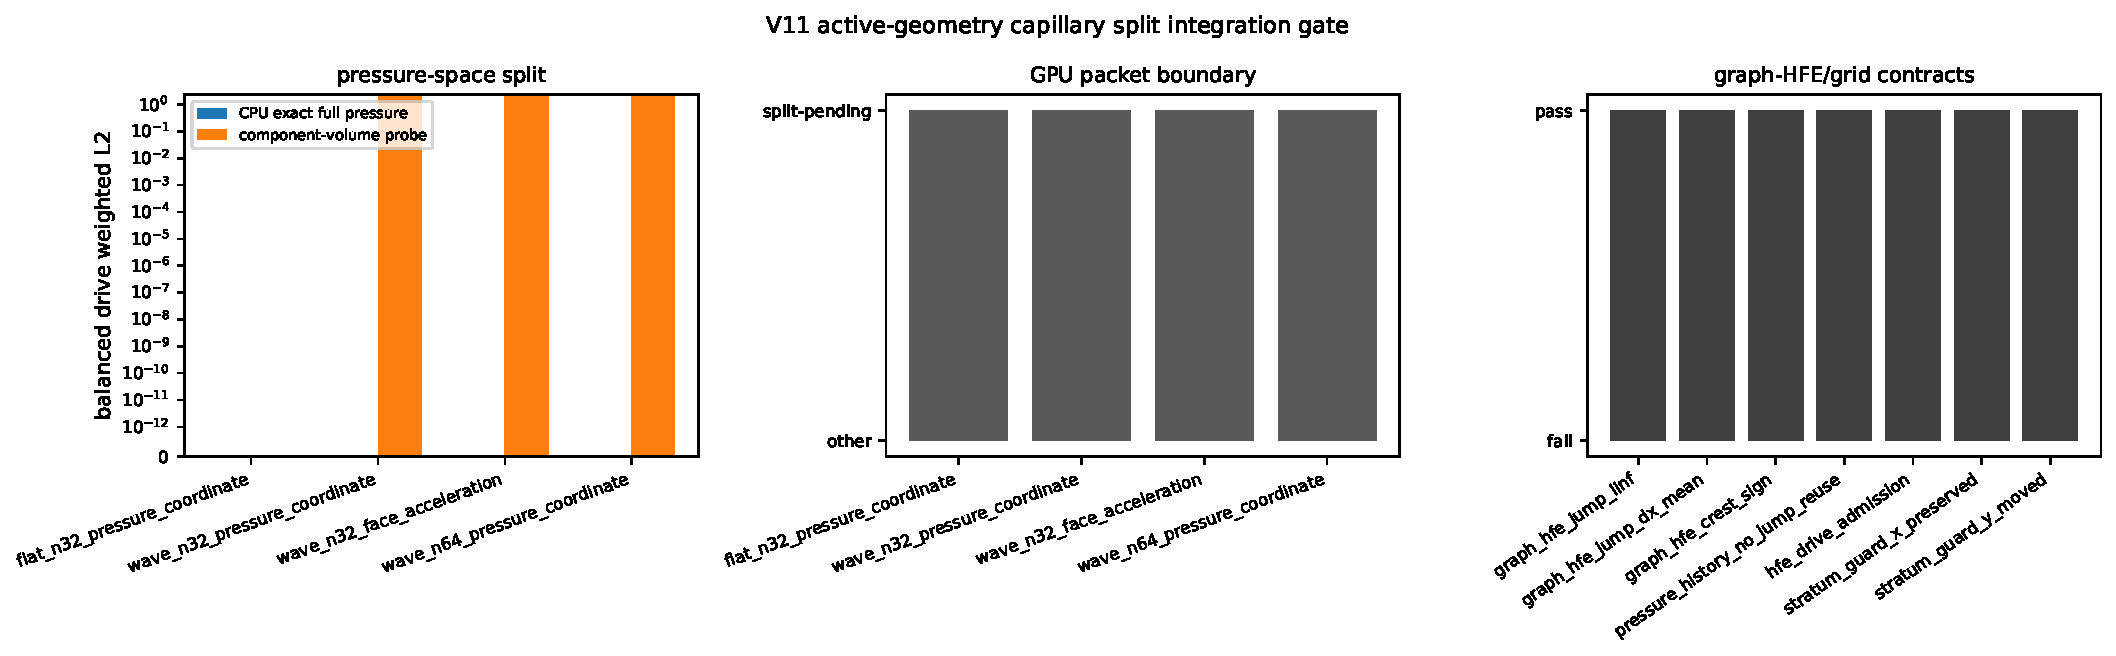
\includegraphics[width=0.78\linewidth]{figures/ch13_v11_ao_capillary_split_gate.pdf}
\caption{V11：アクティブ幾何毛管分解の統合ゲート．
圧力座標と面加速度の履歴表現を含め，
非静的波では全圧力像への過射影を棄却し，最終 $R_p$ 契約へ進めることを確認する．}
\label{fig:V11_ao_gate}
\end{figure}

\paragraph{第14章への接続．}
V11 は，過射影で非静的駆動を消す古い分解を棄却し，
第~\ref{sec:ao_fast_state_space}節の採用条件を本番経路の境界として固定する．
したがって第~\ref{sec:val_capillary}節の毛管波は，
幾何セル分率，bundle Young--Laplace work，pressure-component Hodge reaction，
Hodge 逆適用済み面補間，$q$ 所有グラフ HFE，投影済み面共鎖保存，
正則層ガード，および pressure-coordinate history を同時に使う
アクティブ幾何毛管分解の物理ベンチマークとして読む．
ただし，U12 が棄却した全圧力像への過射影や，
面共鎖移送を欠く節点速度再構成経路は，本節の合格経路ではない．

% paper/sections/13f_error_budget.tex
%
% V1-V11 横断の精度バジェット総合
% Hosts labels: sec:error_budget, sec:accuracy_summary
% (tab:accuracy_summary 09f, sec:time_accuracy_table 07 を authoritative とし
%  本節からは hosting せず外部参照のみで連結する)
% ═══════════════════════════════════════════════════════════════════════════════
\subsection{精度バジェット：V1--V11 誤差寄与の統合評価}
\label{sec:error_budget}
\label{sec:accuracy_summary}

\paragraph{構成．}
本節は V1--V11 横断の精度結果を一表に集約し，
\textbf{各誤差源} (空間離散，時間離散，界面表現，曲率推定，CLS 再初期化，射影後面速度，履歴圧力) と
\textbf{各設定パラメータ} ($\rho_r$, $\alpha$, $\Delta t$, $h$) の関係を整理する
（観測収束次数の Richardson 外挿運用は~\cite{Roy2003}）．
本節は，最終スキームについて，
どの誤差源がどの検証問題で支配的になるかを整理する精度バジェットである．
U10/U11 は第~\ref{sec:numerical_integrity}章の単体条件として扱い，
U12/V11 はアクティブ幾何毛管分解の統合前ゲートとして扱う．
保存形共通フラックスの有限振幅物理応答と周期壁上昇気泡応答は，
第~\ref{sec:benchmarks}章のベンチマークと事前適合性確認で扱う．

\paragraph{判定基準（§\ref{sec:verification} Type 分類との整合）．}
本節は §\ref{sec:verification}「判定区分と Type 分類」に基づき
Type-A/Type-B/Type-D の三類型で各 V テストの判定を集約する
（凡例は表~\ref{tab:V_verdict_types}）．
V1-a, V1-b, V2, V4, V5 は \textbf{Type-A 判定基準}：
連続方程式または単体要素の理想化次数ではなく，
実際に測定する縮約離散恒等関係に対する文献根拠付き判定基準で評価する．
V1-a は単相 TGV 空間の FVM PPE 結合系に対する $O(h^2)$ 傾向，
V1-b は非増分の標準 PPE 射影の $O(\Delta t)$ 傾向，
V2 は壁片側 Kovasznay 統合残差の $O(h^4)$ 傾向，
V4 は固定壁一様オフセット診断の $O(\|\bU\|)$ 有界残差，
V5 は CCD 寄生流れ絶対値 $u_\infty^{\mathrm{end}}$ の $\sigma/\mathrm{Re}_c$ スケール基準
を合格基準とする．
V10-a 質量保存軸 / V10-b 質量保存軸は \textbf{Type-B}：
Olsson--Kreiss 質量補正~\cite{OlssonKreiss2005} を 10 step ごとに適用する
構造的アルゴリズム修正による合格化．
V7（毛管圧力ジャンプ/射影の界面帯に律速され $2.0$ に届かない結合系収束率），V10-a 形状軸（固定格子 CLS 位相/しきい値化誤差 + slot/h$=6.4$ 解像不足），
V10-b 形状軸（格子幅まで薄くなる folded filament の Eulerian 固定格子限界）は \textbf{Type-D}：
連続方程式・離散構造に由来する理論的下限と整合するものとして
条件付き合格 ($\triangle$)．これらは格子増強だけで合格化するのではなく，
norm 切替，項別誤差分解，dt/h 独立掃引，時系列解析により
保証範囲を別途定める必要がある．
V9 は Type-A/B/D の分類ではなく，圧力ジャンプ・毛管射影結合系と同時に基準/局所
$\varepsilon$ 幅を切り替えても有限時間静止液滴を破綻させないことを測る
\textbf{演算子群条件付き診断}として別枠で扱う．
V11 も Type-A/B/D ではなく，アクティブ幾何毛管分解を標準物理経路へ入れる前の
\textbf{採用境界ゲート}として別枠で扱う．

\paragraph{統合検証成績一覧．}

\begin{table}[!ht]
\caption{V1--V11：統合精度まとめ}
\label{tab:v_accuracy_summary}
\PaperCaptionNote{収束率は log-log fitting (3 点以上)；単一値はその設定での代表値．本表は Chapter 12 の成果総括表~\ref{tab:verification_summary} と同じ「ID / テスト / 期待・判定基準 / 実測・観測値 / 判定」文法で読む．表~\ref{tab:U_summary} は成果表ではなく U 系列の検証設計マップである．V10-a/V10-b は質量保存軸 (Type-B) と形状軸 (Type-D) に分離するため，表~\ref{tab:V_summary} の V10-a/b から 1:2 に展開される（V11 ゲートを含め計 15 行）．補助観測指標および全観測指標の網羅的列挙は表~\ref{tab:V_summary} を参照．}
\centering
\PaperTableExtraDenseSetup
\begin{tabularx}{\linewidth}{@{}>{\raggedright\arraybackslash}p{0.10\linewidth}>{\raggedright\arraybackslash}p{0.18\linewidth}>{\raggedright\arraybackslash}p{0.23\linewidth}>{\raggedright\arraybackslash}X>{\raggedright\arraybackslash}p{0.15\linewidth}@{}}
\toprule
ID & テスト & \shortstack{期待・判定\\基準} & \shortstack{実測・観測\\値} & 判定 \\
\midrule
V1-a & 単相 TGV 空間 & FVM PPE 結合系の $O(h^2)$ 傾向 & slope($E_{\mathrm{rel}}, h$) $=\mathbf{2.00}$；$E_{\mathrm{rel}}=1.583\times 10^{-7}$ at $N=64$ & \checkmark Type-A \\
V1-b & 単相 TGV 時間 & 標準 PPE の $O(\Delta t)$ 傾向 & slope($E_{\mathrm{rel}}, \Delta t$) $=\mathbf{1.00}$ & \checkmark Type-A \\
V2 & Kovasznay 空間残差 & 壁片側残差 $O(h^4)$ & slope($\|R\|_\infty, h$) $=\mathbf{3.95}$ & \checkmark Type-A \\
V3 & 静止液滴 long-term & BF 平衡 + 標準構成静止判定 & $|\Delta p_{\mathrm{rel}}|=0.97\%$ at $N=128$；標準構成 $N=32,T=10$: $K_{\max}=1.72\!\times\!10^{-6}$, $|\Delta V|/V_0\le2.92\!\times\!10^{-15}$, $D=0$ & \checkmark \\
V4 & 一様オフセット残差 & $O(\|\bU\|)$ 有界残差，運用上限 $<3$ & $\|\Delta u\|_\infty^{\max}/\|\bU\|=2.63$ & \checkmark Type-A \\
V5 & 寄生流れ 200 step & CCD $u_\infty^{\mathrm{end}}$ の $\sigma/\mathrm{Re}_c$ スケール基準 & $1.93\!\times\!10^{-2}$ at $\rho_r=1,N=32$；FD 比 $1/5.44$ 補助 & \checkmark Type-A \\
V6 & 密度比掃引 & ブローアップなし；CLS 体積ドリフトは丸め誤差床；毛管面バランス & 全 8 ケース安定；$u_\infty^{\mathrm{end}}\le1.3\!\times\!10^{-9}$；$|\Delta V_\psi|/V_{\psi,0}\le1.2\!\times\!10^{-16}$ & \checkmark \\
V7 & IMEX-BDF2 二相時間 & 毛管圧力ジャンプ/射影の界面帯制約下の結合系実効収束率 & slope($\|e\|_\infty,\Delta t$) $=\mathbf{1.59}$ & $\triangle$ Type-D \\
V8 & 非一様 NS 静止 & 非一様 BF 静止判定基準 & $|\Delta p_{\mathrm{rel}}|=2.86\%$ at $\alpha=2,N=96$ & \checkmark \\
V9 & 基準/局所 $\varepsilon$ 切替 & 圧力ジャンプ・毛管射影結合系同時使用下の有界性診断 & B/C=$1.00$ at $N=32$；$u_\infty^{\max}\le9.82\!\times\!10^{-10}$；$|\Delta V|/V_0\le4.73\!\times\!10^{-16}$ & \checkmark 結合系診断 \\
V10-a-mass & Zalesak 質量保存軸 & Olsson--Kreiss 質量補正後 drift $<0.5\%$ & $4.70\!\times\!10^{-4}\%$ at $N=128$ & \checkmark Type-B \\
V10-a-shape & Zalesak 形状軸 & 固定格子位相/しきい値化誤差 + slot/h$=6.4$ 解像不足と整合 & centroid err $4.911\!\times\!10^{-3}$；shape $L^1=8.307\!\times\!10^{-3}$ & $\triangle$ Type-D \\
V10-b-mass & 単一渦 reversal 質量保存軸 & Olsson--Kreiss 質量補正後 drift $<0.5\%$ & $0.0428\%$ at $N=128,T=8$ & \checkmark Type-B \\
V10-b-shape & 単一渦 reversal 形状軸 & 格子幅まで薄くなる folded filament の Eulerian 固定格子下限と整合 & $L^1$ reversal error $=2.248\times10^{-2}$ & $\triangle$ Type-D \\
V11 & アクティブ幾何毛管分解ゲート & 全圧力像への過射影を棄却し，$R_p$ 未確定の分解を標準経路へ入れない & 厳密全圧力分解は毛管波駆動 $0$；成分体積 Hodge 診断は N32/N64 $2.1176/2.3055$；未受理分解は標準経路から分離 & \checkmark ゲート \\
\bottomrule
\end{tabularx}
\end{table}

\FloatBarrier

\paragraph{誤差源の整理．}
\begin{enumerate}\setlength{\itemsep}{0pt}
  \item \textbf{空間離散誤差}．CCD 内点 6 次設計に対し，V2 Kovasznay residual は
        壁片側二階微分境界閉包と大域コンパクト結合により実効 $3.95$．
        Type-A 判定基準 $O(h^4)$ を満たす．TGV では時間誤差床下に到達するため空間収束率は飽和．
  \item \textbf{時間離散誤差}．単相 NS の AB2 predictor は単体 $O(\Delta t^2)$ 設計だが，
        V1-b は標準射影結合を測るため，合格基準は $O(\Delta t)$ 傾向である．
        二相結合では毛管圧力ジャンプ / アフィン FCCD 射影の界面帯誤差が
        結合系実効収束率 $1.59$（V7; \autoref{sec:imex_bdf2_twophase_time}）を支配し，
        純粋 BDF2 2 次ではなく毛管結合系の実効次数として扱う．
  \item \textbf{界面表現誤差}．Heaviside--$\delta$ の基準/局所 $\varepsilon$ 切替は
        FCCD, HFE, 圧力ジャンプ PPE, 毛管成分の圧力勾配射影，射影後面速度閉包，アフィン圧力履歴面加速度と同時に使う条件で有限時間安定（V9）；
        ただしこの direct-$\psi$/HFE 確認では B/C が同一で，局所幅を独立した改善機構とは主張しない．
        CCD/CSF 縮約経路の結果は圧力ジャンプ/HFE 結合系の精度根拠には用いない．
        さらに射影後面速度閉包を用いる結合系では，
        $\psi$ 移流の速度表現そのものが誤差源になりうる．
        射影で得た正準面速度を節点へ再構成してから面フラックスを作り直す経路は，
        式~\eqref{eq:projection_native_psi_transport} の保存則と同値ではないため，
        static-interface の $\psi$ 摂動を曲率誤差へ増幅する．
        同じ理由で，affine-jump IPC の履歴圧力項も
        不連続な $p^n$ を節点スカラーとして微分するのではなく，
        式~\eqref{eq:affine_pressure_history_faces} の正準面加速度として保持する必要がある．
  \item \textbf{射影残差誤差と圧力代表誤差の分離}．
        DC 反復回数そのものは精度証明ではなく，
        式~\eqref{eq:ppe_dc_residual_contract} の高次残差が射影受理条件である．
        したがって圧力ジャンプ PPE の精度評価では，
        楕円求解残差，投影後発散，圧力代表の選択を別々の観測量として扱う．
        残差受理条件を満たした後に残る界面帯圧力振動は，
        直ちに運動量圧力仕事の破綻とは解釈しない．
        affine-jump 経路の物理仕事は面共鎖
        $A_f(G_fp-B_f(j))$ で定義されるため，
        拡散界面帯の未補正節点圧力は Hodge 代表または相内代表に写してから読む．
        壁付き面速度状態空間については U11 が
        $C_wP_w=0$，計量自己随伴性，制限 Green 恒等式，および
        壁/周期壁商空間の階数条件を丸め誤差まで確認したため，
        V6/V7/V9 の圧力ジャンプ/HFE 統合診断はこの単体条件の上で読む．
        ただし U11 は小型代数条件であり，周期壁の有限振幅物理応答を
        第13章に追加するものではない．
  \item \textbf{アクティブ幾何毛管分解の圧力反力分解ゲート}．V11 は，
        式~\eqref{eq:capillary_pressure_reaction_projection} の $R_p$ を定めない
        全圧力像への分解が，毛管波の面上駆動を代数的に消し得ることを
        統合前に検出する．成分体積 Hodge 診断は非静的波の検出器として有用だが，
        それ自体は最終 $R_p$ の代替証明ではない．したがって $R_p$ 未確定の分解は
        未受理とし，標準圧力ジャンプ経路の V6/V7/V9 と第~\ref{sec:benchmarks}章の
        毛管波結果から分離する．
  \item \textbf{曲率推定誤差}．V5 では CSF $\kappa_{lg}$ + CCD 勾配の
        $u_\infty^{\mathrm{end}}$ 絶対値が全表ケースで $2\times10^{-2}$ 以下に保たれ，
        参照として FD 値を全条件で下回る．
        粗格子・低密度比ほど CCD/FD の差は大きい．
  \item \textbf{CLS 形状追跡誤差（質量保存軸 vs 形状精度軸の分離）}．V10 の Zalesak は
        $\alpha=1$ の一様格子診断に固定する．Olsson--Kreiss 質量補正~\cite{OlssonKreiss2005}
        を 10 step ごとに適用した結果，$N=128$ で質量ドリフト $4.70\times 10^{-4}\%$（合格基準
        $0.5\%$ を 3 桁下回り \checkmark）に到達する一方，centroid err $4.911\times 10^{-3}$,
        shape $L^1$ $8.307\times 10^{-3}$, 重心収束率 $\approx 1.22$ は固定格子
        CLS 位相/しきい値化誤差と slot/h $=6.4$ の sharp-corner 解像不足に
        律速される．単一渦 (V10-b) も同質量修正下で
        質量ドリフト $0.0428\%$ \checkmark / $L^1$ reversal $2.248\times10^{-2}$ ($T=8$ の
        格子幅 folded filament に対する Eulerian 固定一様格子の理論的下限~\cite{EnrightFedkiwFerzigerMitchell2002}) と
        同じく\textbf{保存軸 \checkmark / 形状軸 $\triangle$} の二軸構造を取る．
  \item \textbf{判定軸の分離}．V7/V10 系は単一の設計次数だけで判定せず，
        毛管/射影結合，固定格子 CLS 形状誤差，および
        質量補正後の保存軸を分けて読む．
\end{enumerate}

\paragraph{合格判定要約（§\ref{sec:verification} Type 分類で集約）．}
\begin{itemize}\setlength{\itemsep}{0pt}
  \item \checkmark \textbf{合格（設計基準）}:
        V3 (BF 平衡，$|\Delta p_{\mathrm{rel}}|=0.97\%$ at $N=128$；標準構成静止判定で $K_{\max}\le1.72\!\times\!10^{-6}$, $|\Delta V|/V_0\le2.92\!\times\!10^{-15}$, $D=0$)，
        V6 (密度比ロバスト, $\rho_r=833$ までブローアップなし; $u_\infty^{\mathrm{end}}\le1.3\!\times\!10^{-9}$; $|\Delta V_\psi|/V_{\psi,0} \le 1.2\!\times\!10^{-16}$)，
        V8 (非一様静止, $\alpha=2,N=96$ で $|\Delta p_{\mathrm{rel}}|=2.86\%$).
  \item \checkmark \textbf{Type-A 判定基準合格}:
        V1-a (TGV 空間 FVM PPE $O(h^2)$ 傾向, 細格子側局所収束率 $2.00$；補助: $E_{\mathrm{rel}}=1.583\!\times\!10^{-7}$ at $N=64$)，
        V1-b (標準射影結合 $O(\Delta t)$ 傾向, 収束率 $1.00$)，
        V2 (Kovasznay 壁残差 $O(h^4)$ 傾向, 収束率 $3.95$)，
        V4 (固定壁一様オフセット $O(\|\bU\|)$ 有界残差, $\|\Delta u\|_\infty^{\max}/\|\bU\| = 2.63$)，
        V5 (CCD 寄生流れ絶対値 $1.93\!\times\!10^{-2}$ at $\rho_r=1, N=32$).
  \item \checkmark \textbf{Type-B 構造修正 合格}:
        V10-a 質量保存軸 (Olsson--Kreiss 質量補正; $N=128$ 質量ドリフト $4.70\!\times\!10^{-4}\%$)，
        V10-b 質量保存軸 (同; $0.0428\%$).
  \item $\triangle$ \textbf{Type-D 理論的下限との整合}:
        V7 (二相結合系の実効収束率 $1.59$ — 毛管圧力ジャンプ/射影
        界面帯に律速され，BDF2 単体 $2.0$ には届かない),
        V10-a 形状軸 ($\alpha=1$ Zalesak centroid err $4.911\times 10^{-3}$,
        shape $L^1$ $8.307\times 10^{-3}$ — 固定格子 CLS 位相/しきい値化誤差と
        slot/h $=6.4$ sharp-corner 解像不足律速),
        V10-b 形状軸 ($T=8$ 単一渦 reversal $L^1=2.248\times10^{-2}$
        — 格子幅 folded filament の Eulerian 固定格子原理的下限~\cite{EnrightFedkiwFerzigerMitchell2002}).
  \item $\times$ \textbf{要改善 / 推奨せず}: 該当なし.
  \item \checkmark \textbf{演算子群条件付き診断}: V9
        (基準/局所 $\varepsilon$ 切替は $N=32$ で B/C=$1.00$，$u_\infty^{\max}\le9.82\!\times\!10^{-10}$，$|\Delta V|/V_0\le4.73\!\times\!10^{-16}$；
        HFE 曲率 + 圧力ジャンプ PPE + 毛管成分の圧力勾配射影 + 射影後面速度閉包 + アフィン圧力履歴面加速度と同時使用しても有限時間静止液滴を破綻させないが，
        局所幅の改善効果はこの縮約確認では主張しない).
\end{itemize}

\paragraph{設計指針 (PR-5 Algorithm Fidelity)．}
\begin{itemize}\setlength{\itemsep}{0pt}
  \item 単相 NS：CCD 内点 6 次空間 + AB2 predictor 2 次時間設計は単体レベルで維持する．
        統合縮約実験では，Kovasznay 壁残差は $O(h^4)$，
        標準 PPE TGV 時間傾向は $O(\Delta t)$ として判定する．
  \item 二相 NS：圧力ジャンプ・毛管射影結合系
        （分相 PPE + DC + HFE + 毛管成分の圧力勾配射影 + 射影後面速度閉包 + アフィン圧力履歴面加速度）が
        密度比 $\le 833$ でロバスト（V6）．
        ただし時間方向の実効次数は界面処理に律速されるため，
        \textbf{$\Delta t$ を $h_{\min}$ より小さく取る安全ファクタ}（CFL $\le 0.4$）が推奨．
  \item 非一様格子：$\alpha>1$ の NS 静止問題と基準/局所 $\varepsilon$ 切替は V8/V9 で検証し，
        Zalesak slot と単一渦 reversal は $\alpha=1$ の一様格子 CLS 移流診断に固定する．
        局所幅を改善根拠として用いるには，移動界面または再初期化が局所厚みを
        実際に経由する別検証を要求する．
  \item 寄生流れ抑制：CCD の $u_\infty^{\mathrm{end}}$ 絶対値は V5 全表ケースで
        $O(10^{-2})$ 以下に保たれ，代表的には
        $\rho_r=1,N=32$ で $1.93\!\times\!10^{-2}$，$\rho_r=1,N=128$ で $6.28\!\times\!10^{-4}$．
        参照として FD 値を全条件で下回り（$\rho_r=1,N=32$ で $1/5.44$，
        $\rho_r=100,N=64$ で $1/2.5$），高解像度・高密度比では CCD/FD 差が縮小する．
\end{itemize}

\paragraph{検証対応の統合．}
本節は V1--V11 全結果の横断統合点である．各実験が測定した式・離散化・物理指標の対応を
以下に集約する：
\begin{itemize}\setlength{\itemsep}{0pt}
  \item V1 (\autoref{sec:single_phase_ns}) — Navier--Stokes \eqref{eq:NS_onefluid}
        と AB2 + 標準 PPE 縮約経路に対するエネルギー減衰と非圧縮残差．
  \item V2 (\autoref{sec:single_phase_ns}, \autoref{sec:kovasznay}) —
        CCD 内点 6 次演算子と壁片側境界閉包を含む Kovasznay 統合残差．
  \item V3, V5 (\autoref{sec:bf_static_droplet}, \autoref{sec:spurious_multistep})
        — BF 力学的バランス \eqref{eq:bf_fccd_unification} + CSF
        \eqref{eq:csf_final} に対する Laplace 圧維持と寄生流れ，および
        圧力ジャンプ/Riesz 標準構成の静止判定による幾何・体積保持．
  \item V4 (\autoref{sec:galilean_offset}) —
        固定壁系の一様オフセット残差に対する $O(\|\bU\|)$ 有界性．
  \item V6, V7 (\autoref{sec:density_ratio_sweep},
        \autoref{sec:imex_bdf2_twophase_time}) — 圧力ジャンプ・毛管射影結合系
        （分相 PPE \eqref{eq:split_ppe} + DC + HFE + 毛管成分の圧力勾配射影 +
        射影後面速度閉包 + アフィン圧力履歴面加速度）に対する密度比安定性と二相時間精度．
  \item V8 (\autoref{sec:nonuniform_ns_static}) — 非一様 NS に対する静止液滴
        $\Delta p_{\mathrm{rel}}$ 維持．
  \item V9 (\autoref{sec:local_eps_validation}) — 圧力ジャンプ・毛管射影結合系上の基準/局所 $\varepsilon$ 切替に対する
        寄生流れ，体積分率ドリフト，および B/C 同一性．
  \item V10-a (\autoref{sec:zalesak_cls_advection}) — Zalesak CLS 移流に対する
        質量ドリフトと centroid 追跡精度（質量保存軸 / 形状軸の二軸構造）．
  \item V10-b (\autoref{sec:single_vortex_reversal}) — 単一渦 deformation
        reversal に対する $L^1$ 誤差と質量ドリフト（同二軸構造）．
  \item V11 (\autoref{sec:ao_fast_capillary_gate}) — アクティブ幾何毛管分解の
        全圧力像への過射影反例，成分体積 Hodge 診断，標準経路への採用境界．
\end{itemize}
本節 \autoref{tab:v_accuracy_summary} はこの全対応の精度結果を一表に集約する
唯一の総合表であり，他章 (\autoref{sec:conclusion}) からの参照は
本表をエンドポイントとする．

\FloatBarrier

